
%
% The PSI Programmer's Manual
%

\documentclass[12pt]{article}
% Use this if you need to include PostScript figures or such.
%\usepackage{epsfig}
\usepackage{html}
\usepackage{epsfig}
\usepackage{graphicx}
\setlength{\textheight}{9in}
\setlength{\textwidth}{6.5in}
\setlength{\hoffset}{0in}
\setlength{\voffset}{0in}
\setlength{\headheight}{0in}
\setlength{\headsep}{0in}
\setlength{\topmargin}{0in}
\setlength{\oddsidemargin}{-0.05in}
\setlength{\evensidemargin}{-0.05in}
\setlength{\marginparsep}{0in}
\setlength{\marginparwidth}{0in}
\setlength{\parsep}{0.8ex}
\setlength{\parskip}{1ex plus \fill}
\baselineskip 18pt
\renewcommand{\topfraction}{.8}
\renewcommand{\bottomfraction}{.2}

\begin{document}

%%%%%%%%%%%%%%%%%%%%%%%
% Definitions
%%%%%%%%%%%%%%%%%%%%%%%

\newcommand{\PSItwo}{{\tt PSI2}}
\newcommand{\PSIthree}{{\tt PSI3}}

%
% Psi Modules
%
\def\module#1{{\tt #1}}
\newcommand{\PSIdriver}{\module{psi}}
\newcommand{\PSIinput}{\module{input}}
\newcommand{\PSIcints}{\module{cints}}
\newcommand{\PSIcderiv}{\module{cints --deriv1}}
\newcommand{\PSIdetci}{\module{detci}}
\newcommand{\PSIdetcas}{\module{detcas}}
\newcommand{\PSIdetcasman}{\module{detcasman}}
\newcommand{\PSIclag}{\module{clag}}
\newcommand{\PSIccenergy}{\module{ccenergy}}
\newcommand{\PSIccsort}{\module{ccsort}}
\newcommand{\PSIpsi}{\module{psi}}
\newcommand{\PSIcscf}{\module{cscf}}
\newcommand{\PSIoptking}{\module{optking}}
\newcommand{\PSItransqt}{\module{transqt}}
\newcommand{\PSInormco}{\module{normco}}
\newcommand{\PSIintder}{\module{intder95}}
\newcommand{\PSIgeom}{\module{geom}}
\newcommand{\PSIoeprop}{\module{oeprop}}

%
% Psi Library
%
\def\library#1{{\tt #1}}

%
% Psi and Unix Files
%
\def\FILE#1{{\tt file#1}}
\def\file#1{{\tt #1}}
\newcommand{\inputdat}{\file{input.dat}}
\newcommand{\outputdat}{\file{output.dat}}
\newcommand{\fconstdat}{\file{fconst.dat}}
\newcommand{\intcodat}{\file{intco.dat}}
\newcommand{\optaux}{\file{opt.aux}}
\newcommand{\basisdat}{\file{basis.dat}}
\newcommand{\pbasisdat}{\file{pbasis.dat}}
\newcommand{\geomdat}{\file{geom.dat}}
\newcommand{\geomout}{\file{geom.out}}

%
% Psi Keywords
%
\def\keyword#1{{\tt #1}}

%
% Psi C and Fortran Language elements
%
\def\celem#1{{\tt #1}}
\def\felem#1{{\tt #1}}

%
% Unix stuff
%
\def\unixid#1{{\em #1}} % names of groups and users
\def\shellvar#1{{\tt #1}}

%
% Nice output for function description
%
% Needs 4 arguments: function declaration,
%  description, arguments, and return values
%
% Call \initfuncdesc before using \funcdesc
%
\newcommand{\initfuncdesc}
{\newlength{\lcwidth}
\settowidth{\lcwidth}{Arguments:}
\newlength{\rcwidth}
\setlength{\rcwidth}{\linewidth}
\addtolength{\rcwidth}{-1.0\lcwidth}
\addtolength{\rcwidth}{-6.0\tabcolsep}
}

\newcommand{\funcdesc}[4]{
\celem{#1} \\
#2

\begin{tabular}{lp{\rcwidth}}
Arguments: & #3\\
Returns: & #4
\end{tabular}}


\initfuncdesc

\begin{center}
\ \\
\vspace{2.0in}
{\bf {\Large The \PSIthree\ Programmer's Manual}} \\
\vspace{0.5in} 
T. Daniel Crawford,$^a$ C. David Sherrill,$^b$ Edward F.\ Valeev,$^{a}$ \\
Justin T. Fermann,$^c$ and C. Brian Kellogg$^c$ \\ 
\ \\ 
{\em $^a$Department of Chemistry, Virginia Tech, Blacksburg, Virginia 24061} \\
\vspace{0.1in}
{\em $^b$Center for Computational Molecular Science and Technology, 
\mbox{Georgia Institute of Technology,} Atlanta, Georgia 30332-0400} \\
\vspace{0.1in}
{\em $^c$Center for Computational Quantum Chemistry, \\ 
\mbox{University of Georgia,} Athens, Georgia 30602-2525} \\
\ \\
\vspace{0.3in}
\PSIthree\ Version: \PSIversion \\
Created on: \today \\
Report bugs to: \PSIemail \\
\end{center}

\thispagestyle{empty}

\newpage
\tableofcontents

\newpage
\section{Introduction}
%
% History of Psi
%
% Daniel Crawford, 24 January, 1996
%

The PSI suite of {\em ab initio} quantum chemistry programs is the result
of an ongoing attempt by a cadre of graduate students, postdoctoral
associates, and professors to produce code that is efficient but also
easy to extend to new theoretical methods.  Significant effort has been
devoted to the development of libraries which are robust and easy to use.
Some of the earliest contributions to what is now referred to as ``PSI''
include a direct configuration interaction (CI) program (Robert Lucchese,
1976, now at Texas A\&M), the well-known graphical unitary group CI program
(Bernie Brooks, 1977-78, now at N.I.H.), and the original integrals code
(Russ Pitzer, 1978, now at Ohio State).  From 1978-1987, the package was
know as the {\tt BERKELEY} suite, and after the Schaefer group moved to the
Center for Computational Quantum Chemistry at the University of Georgia,
the package was renamed {\tt PSI}.  Thanks primarily to the efforts of Curt
Janssen (Sandia Labs, Livermore) and Ed Seidl (LLNL), the package was
ported to UNIX systems, and substantially improved with new input formats
and a C-based I/O system.

Beginning in 1999, an extensive effort was begun to develop \PSIthree\
--- a {\tt PSI} suite with a completely new face.  As a result of this
effort, all of the legacy Fortran code was removed, and everything was
rewritten in C and C++, including new integral/derivative integral,
coupled cluster, and CI codes.  In addition, new I/O libraries have
been added, as well as an improved checkpoint file structure and greater
automation of typical tasks such as geometry optimization and frequency
analysis.  The package has the capability to determine wavefunctions,
energies, analytic gradients, and various molecular properties based on
a variety of theories, including spin-restricted, spin-unrestricted, and
restricted open-shell Hartree-Fock (RHF, UHF, and ROHF); configuration
interaction (CI) (including a variety of multireference CI's and full
CI); coupled-cluster (CC) including CC with variationaly optimized
orbitals; second-order M{\o}ller-Plesset perturbation theory (MPPT)
including explicitly correlated second-order M{\o}ller-Plesset energy
(MP2-R12); and complete-active-space self-consistent field (CASSCF)
theory.  By January 2008, all of the C code in \PSIthree\ was 
converted to C++ to enable a path toward more object-oriented design
and a single-excecutable framework that will facilitate code reuse and 
ease efforts at parallelization.  At this same time, all of the legacy I/O
routines from {\tt PSI2} were removed, greatly streamlining the
\library{libciomr.a} library.


\section{Introduction} \label{introduction}

\subsection{Overview} 

This manual explains how to use the \PSIthree\ suite of {\em ab initio}
quantum chemical programs.  In this section, we provide an overview of
some of the features of \PSIthree\ along with the prerequisite steps for
running calculations.  Section \ref{tutorial} provides a brief tutorial to
help new users get started.  Section \ref{input} offers further details
into the structure of \PSIthree\ input files and a discussion of some of
the most important options.  Later sections deal with the different types
of computations which can be done using \PSIthree\ (e.g., Hartree-Fock,
MP2, coupled-cluster) and general procedures such as geometry optimization
and vibrational frequency analysis.  The appendix will eventually include a
description of the input keywords and command-line options for each module,
as well as numerous examples of \PSIthree\ input and basis set files.
For the latest \PSIthree\ documentation, check \htmladdnormallink{{\tt
www.psicode.org}} {http://www.psicode.org/}.

The \PSIthree\ package was developed to perform high-accuracy quantum
mechanical computations on challenging chemical species and to provide an
infrastructure for the development of new theoretical techniques.  Hence,
it has a very flexible input scheme which allows non-standard computations,
and it is easily adapted to enable new capabilities.

The following citation should be used in any publication utilizing the
\PSIthree\ program package:

\begin{quotation}
\noindent
T. Daniel Crawford, C. David Sherrill, Edward F. Valeev, Justin
T. Fermann, Rollin A. King, Matthew L. Leininger, Shawn T. Brown,
Curtis L. Janssen, Edward T. Seidl, Joseph P. Kenny, and Wesley D. Allen,
{\em J. Comput. Chem.}, in press.

\end{quotation}

\subsection{Obtaining and Installing \PSIthree}
\label{installation}

The latest version of the \PSIthree\ program package may be obtained at
\htmladdnormallink{{\tt www.psicode.org}}{http://www.psicode.org}.  The
source code is available as a gzipped tar archive (named, for example, {\tt
psi3.X.tar.gz}), and binaries may be available for certain architectures.
For detailed installation and testing instructions, please refer to the
the \PSIthree\ Installation Manual, available as part of the package or
at the \PSIthree\ website above.

\subsection{Supported Architectures}
The majority of \PSIthree\ was developed on IBM RS/6000/AIX
and x86/GNU Linux workstations. The complete list of
tested architectures to which \PSIthree\ has
been ported is shown in Table \ref{table:ports}.
\begin{table}[h]
\caption{Platforms on which \PSIthree\ has been installed successfully.}
\label{table:ports}
\begin{center}
\begin{tabular}{ll} \hline\hline
Architecture              &  Notes \\ \hline
Compaq Alpha Tru64 UNIX   & 64-bit mode \\
IBM AIX 4.3.3, 5.x on PowerPC & 64-bit mode \\
Linux on Intel/AMD x86, AMD x86-64  & 32 and 64-bit\\
Apple OS X (Darwin) on PowerPC & \\
SGI IRIX64 ($>$6.5.15)    & 64-bit \\ \hline\hline
\end{tabular}
\end{center}
\end{table}
If you don't find your system in the Table, there's a good chance
that you will be able to install \PSIthree\ on your system
if you have the prerequisite tools and math and utility libraries described 
in the installation manual.

\subsection{Capabilities}
\PSIthree\ can perform {\em ab initio} computations employing
basis sets of up to 32768 contracted Gaussian-type functions of
virtually arbitrary orbital quantum number.
\PSIthree\ can recognize and exploit the largest Abelian subgroup of the
point group describing the full symmetry of the molecule.
Table \ref{table:methods} displays the range of theoretical
methods available in \PSIthree .

\begin{table}
\caption{Summary of theoretical methods available in \PSIthree.} \label{table:methods}
\parsep 10pt
\begin{center}
\begin{tabular}{lccc} \hline\hline
Method           & Energy & Gradient & Hessian \\ \hline
RHF SCF          & Y & Y & Y \\
ROHF SCF         & Y & Y & N \\
UHF SCF          & Y & N & N \\
HF DBOC          & Y & N & N \\
CIS/RPA/TDHF     & Y & N & N \\
TCSCF            & Y & Y & N \\
CASSCF           & Y & Y & N \\
RAS-CI           & Y & N & N \\
RAS-CI DBOC      & Y & N & N \\
RHF/UHF/ROHF MP2     & Y & N & N \\
RHF MP2-R12      & Y & N & N \\
RHF/UHF/ROHF CCSD    & Y & Y & N \\
RHF/UHF/ROHF CCSD(T) & Y & N & N \\
RHF EOM-CCSD     & Y & N & N \\
ROHF EOM-CCSD    & Y & N & N \\
\hline\hline
\end{tabular}
\end{center}
\end{table}
Geometry optimization (currently restricted to true minima on the potential
energy surface) can be performed using either analytic gradients
or energy points.  Likewise, vibrational frequencies can be 
computed using analytic second derivatives or by finite
differences of analytic gradients.
\PSIthree\ can also compute an extensive list of one-electron properties.

\subsection{Technical Support} The \PSIthree\ package is
distributed for free and without any guarantee of reliability,
accuracy, suitability for any particular purpose.  No obligation
to provide technical support is expressed or implied.  As time
allows, the developers will attempt to answer inquiries directed to
\htmladdnormallink{{\tt crawdad@vt.edu}}{mailto:crawdad@vt.edu}.
For bug reports, specific and detailed information, with example
inputs, would be appreciated.  Questions or comments regarding
this user's manual may be sent to \htmladdnormallink{{\tt
sherrill@gatech.edu}}{mailto:sherrill@gatech.edu}.





\section{The \PSIthree\ Source Code}\label{cvs}
%
% PSI Programmer's Manual
%
% SVN Revision Control Section
% (formerly CVS)
%
% TDC, February, 1996
% Modified by TDC, December 2002
% Updated from CVS to SVN, April 2007
%

The subversion control system (SVN) (\htmladdnormallink{{\tt
    subversion.tigris.org}}{http://subversion.tigris.org/}) provides a
convenient means by which programmers may obtain the latest (or any
previous) version of the \PSIthree\ source from the main repository or
a branch version, add new code to the source tree or modify existing
\PSIthree\ modules, and then make changes and additions available to
other programmers by checking the modifications back into the main
repository.  SVN also provides a ``safety net'' in that any erroneous
modifications to the code may be easily removed once they have been
identified.  This section describes how to use SVN to access and
modify the \PSIthree\ source code.  (Note that compilation and
installation instructions are given in a separate document.)

The main repository for the \PSIthree\ Source code is currently
maintained by the Crawford group at Virginia Tech.  To check out the
code, one must first obtain an SVN account by emailing
\htmladdnormallink{{\tt crawdad@vt.edu}}{mailto:crawdad@vt.edu}.
After you have a login-id and password, you are now ready to access
the repository via a secure, SSL-based WebDAV connection, but first
you must decide which version of the code you need.

The PSI3 SVN repository contains three top-level directories:
\begin{itemize}
\item {\tt trunk}: The main development area.
\item {\tt branches}: Release branches and private development
  branches are stored here.
\item {\tt tags:} Snapshots of the repository corresponding to public
  releases are stored here and should {\em never} be modified.
\end{itemize}
If you have a PSI3 SVN account, you can peruse these directories if
you like by pointing web browser to:

\noindent
{\tt https://sirius.chem.vt.edu/svn/psi3/}

\subsection{\PSIthree\ CVS Policies: Which Branch Should I Use?}
\label{section:branches}

The \PSIthree\ repository is comprised of a main trunk and several
release branches.  The branch you should use depends on the sort of 
work you plan for the codes:
\begin{enumerate}
\item For any piece of code already in the most recent release, bug
  fixes (defined as anything that doesn't add functionality ---
  including documentation updates) should be made {\em only} on the
  most recent stable release branch.
\item The main trunk is reserved for development of new functionality.
  This allows us to keep new, possibly unstable code away from public
  access until the code is ready.
\item Code that you do not want to put into next major release of
  \PSIthree\ should be put onto a separate branch off the main
  trunk. You will be solely responsible for maintenance of the new
  branch, so you should read the SVN manual before attempting this.
\end{enumerate}

\noindent Fig.~\ref{Fig:svn} provides a schematic of the SVN
revision-control structure and branch labeling.  Two release branches
are shown, the current stable branch, named {\tt psi-3-3}, and a
planned future release, to be named {\tt psi-3-4}.  The tags on the
branches indicate release points, where bugs have been fixed and the
code has been or will be exported for public distribution.  As soon as
a release branch is created, we generate a tag so that we may make
updates to that version of the code without affecting other branches
or the main trunk.  The dotted lines in the figure indicate merge
points: before each public release, changes made to the code on the
stable release branch will be merged into the main trunk.

% We have adopted the convention that the first tag on a new release
% branch will be given the suffix, {\tt -rc-1}, for ``release candidate
% 1'' (i.e., a numbered beta release).  Subsequent tags for new released
% on the same branch will be updated with {\tt -rc-2}, {\tt -rc-3}, etc.
% Once the code is appropriately stable to be beyond beta status,
% release tags will be given the suffix, {\tt -0}, {\tt -1}, etc.,
% indicating patch levels.  


\begin{figure}[h]
\begin{center}
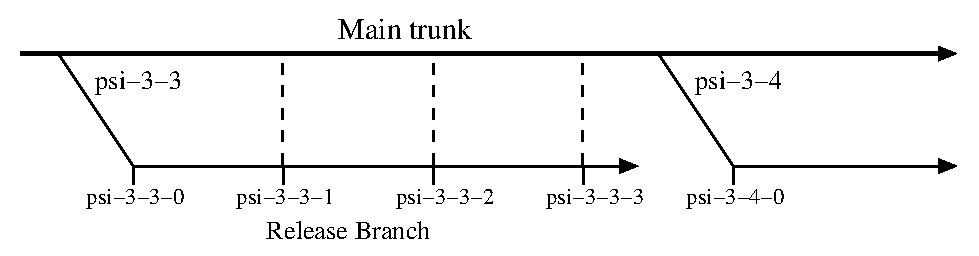
\epsfig{file=svn.eps,height=3.5cm}
\end{center}
\caption{\PSIthree\ SVN branch structure with examples of branch- and
release-tag labelling.}
\label{Fig:svn}
\end{figure}

\noindent A frequently encountered problem is what to do about bug fixes
that are necessary for uninterrupted code development of the code on the
main trunk. As Rule 1 of the above policy states, all bug fixes of the code
already in the recent stable release must go on the corresponding branch,
not on the main trunk. The next step depends on the severity of the bug:
\begin{enumerate}
\item If the bug fix is critical and potentially affects every
  developer of the code on the main trunk, then \PSIthree\
  administrators should be notified of the fix. If deemed necessary,
  appropriate steps to create a new patch release will be made. Once
  the next patch release is created then the bug fixes will be merged
  onto the main trunk.  If the bug fix doesn't warrant an immediate
  new patch release, then you can incorporate the bug fix into your
  local copy of the main trunk code manually or using SVN merge
  features. This will allow you to continue development until next
  patch release is created and the bug fix is incorporated into the
  main trunk code in the repository. However you should {\em never}
  merge such changes into the main trunk yourself.
\item If the bug fix is not critical (e.g. a documentation
  update/fix), then you should wait until next patch release when it
  will be merged into the main trunk automatically.
\end{enumerate}

\noindent
The following are some of the most commonly used SVN commands for checking
out and updating working copies of the \PSIthree\ source code.

\noindent
$\bullet$ To checkout a working copy of the head of the main trunk:

{\tt svn co https://sirius.chem.vt.edu/svn/psi3/trunk/ psi3} 

\noindent
$\bullet$ To check out a working copy of the head of a specific release branch,
e.g., the branch labelled {\tt psi-3-3}:

{\tt svn co https://sirius.chem.vt.edu/svn/psi3/branches/psi-3-3 psi3}

\noindent Note that subsequent {\tt svn update} commands in this
working copy will provide updates only on the chosen branch.  Note
also that after you have checked out a fresh working copy of the code
you must run the {\tt autoconf} command to generate a {\tt configure}
script for building the code.  (See the installation manual for
configuration, compilation, and testing instructions.)

\noindent For each of the above commands, the working copy of your
code will be placed in the directory \file{psi3}, regardless of your
choice of branch.  In this manual, we will refer to this directory
from now on as {\tt \$PSI3}.  Subsequent SVN commands are usually run
within this top-level directory.

\noindent
$\bullet$ To update your current working copy to include the latest revisions:

{\tt svn update}

\noindent
Notes: (a) This will update only the revisions on your current branch;
(b) The old {\tt -d} and {\tt -P} flags required by CVS are not necessary with SVN. 

\noindent
$\bullet$ To convert your working copy to the head of a specific branch:

{\tt svn switch https://sirius.chem.vt.edu/svn/psi3/branches/psi-3-3}

\noindent
$\bullet$ To convert your working copy to the head of the main trunk:

{\tt svn switch https://sirius.chem.vt.edu/svn/psi3/trunk/}

\noindent
$\bullet$ To find out what branch your working copy is on, run this in your
top-level \PSIthree\ source directory:

{\tt svn info | grep URL}

\noindent
This will return the SVN directory from which your working copy was
taken, e.g.,

\noindent
{\tt URL: https://sirius.chem.vt.edu/svn/psi3/branches/psi-3-3}

\noindent
Some words of advice:
\begin{enumerate}
\item Most SVN commands are reasonably safe, 

\item Unlike CVS, you shouldn't use {\tt svn update} to see the status
  of your working copy.  With SVN you should use {\tt svn status} to
  see if you've modified any files or directories.  If you want a
  direct comparison with the repository, you should use {\tt svn status -u}.
\item Read the SVN manual.  Seriously.
\begin{center}
\htmladdnormallink{{\tt
http://svnbook.red-bean.com/en/1.2/svn-book.html}{http://svnbook.red-bean.com/en/1.2/svn-book.html}
\end{center}
\item If you're about to start some significant development or bug-fixes,
first update your working copy to the latest version on your branch.
In addition, if you do development over a long period of time (say weeks to
months) on a specific module or modules, be sure to run a {\tt svn status -u}
occasionally. In can be {\em very} frustrating to try to check in lots
of changes, only to find out that the \PSIthree\ has changed dramatically
since your last update.
\end{enumerate}

\subsection{Checking in altered \PSIthree\ binaries or libraries}

If you have changes to Psi binaries or libraries which already exist, one
of two series of steps is necessary to check these changes in to the main
repository. The first series may be followed if all changes have been made
only to files which already exist in the current version. The second series
should be followed if new files must be added to the code in the repository.

\begin{itemize}
\item No new files need to be added to the repository. We will use
\library{libciomr} as an example. 
\begin{enumerate}
\item {\tt cd \$PSI3/src/lib/libciomr}
\item {\tt svn ci -m ``Put comments here.''}
\end{enumerate}
\item New files must be added to the repository. Again, we use 
\library{libciomr}
as an example. Suppose the new file is named \file{great\_code.c} .
\begin{enumerate}
\item {\tt cd \$PSI3/src/lib/libciomr} 
\item {\tt svn add great\_code.c} 
\item {\tt svn ci -m ``Put comments here.''}
\end{enumerate}
\end{itemize}

The \file{svn ci} command in both of these sequences will examine all
of the code in the current \file{libciomr} directory against the
current version of the code in the main repository. Any files which
have been altered (and for which no conflicts with newer versions
exist!) will be identified and checked in to the main repository (as
well as the new file in the second situation).

SVN requires that you include a comment on your changes.  However,
unlike CVS, SVN prefers that you put your comments on the command-line
rather than editing a text file.  I prefer the CVS way, but this is a
minor pain compared to all the advantages of SVN, in my opinion.

\subsection{Adding entirely new code to the main \PSIthree\ repository} 
\label{checkin_new}

If the programmer is adding a new executable module or library to the
\PSIthree\ repository, a number of important conventions should be followed:

\begin{enumerate}
\item Since such changes almost always involve additional functionality,
new modules or libraries should be added only on the main CVS trunk.
See section \ref{section:branches} for additional information.

\item The directory containing the new code should be given a name
  that matches the name of the installed code (e.g. if the code will
  be installed as \module{newcode}, the directory containing the code
  should be named \file{newcode}). New executable modules must be
  placed in \shellvar{\$PSI3}\file{/src/bin} and libraries in
  \shellvar{\$PSI3}\file{/src/lib} of the user's working copy.

\item The Makefile should be converted to an input file for the
  configure script (\file{Makefile.in} --- see any of the current
  \PSIthree\ binaries for an example) and should follow the
  conventions set up in all of the current \PSIthree\
  \file{Makefiles}. This includes use of \file{MakeVars} and
  \file{MakeRules}.

\item New binaries should be added to the list contained in
  \shellvar{\$PSI3}\file{/src/bin/Makefile.in} so that they will be
  compiled automatically when a full compilation of the \PSIthree\
  distribution occurs. This step is included in the sequence below.

\item A documentation page should be included with the new code (see
  section \ref{Documentation} for more information). As a general
  rule, if the code is not ready to have a documentation page, it is
  not ready to be installed in \PSIthree.

\item The \file{configure.ac} file must be altered so that users may
  check out copies of the new code and so that the \file{configure}
  script will know to create the Makefile for the new code. These
  steps are included in the sequence below.

\end{enumerate}

Assume the new code is an executable module and is named
\module{great\_code}. The directory containing the new code must
contain only those files which are to be checked in to the repository!
Then the following steps will check in a new piece of code to the main
repository:

\begin{enumerate}
\item {\tt cd \$PSI3/src/bin}
\item {\tt svn add great\_code}
\item {\tt svn ci -m ``Put comments here.''}
\item {\tt cd \$PSI3}
\item Edit \file{configure.ac} and add \file{great\_code} to the list. 
\item {\tt svn ci configure.ac -m ``Put comments here.''}
\item {\tt autoconf} 
\item {\tt cd \$PSI3/src/bin} 
\item Edit \file{Makefile.in} and add \file{great\_code} to the list. 
\item {\tt svn ci Makefile.in -m ``Put comments here.''}
\end{enumerate}
At this point, all of the code has been properly checked in, but you
should also test to make sure that the code can be checked out by
other programmers, and that it will compile correctly. The following
steps will store your personal version of the code, check out the new
code, and test-compile it:
\begin{enumerate}
\item {\tt cd \$PSI3/src/bin}
\item {\tt mv great\_code great\_code.bak}
\item {\tt cd \$PSI3/..}
\item {\tt svn update}
\item {\tt cd \$objdir}
\item {\tt \$PSI3/configure -}{\tt -prefix=\$prefix}
\item {\tt cd src/bin/great\_code}
\item {\tt make install}
\end{enumerate}
(Note that \$prefix and \$objdir to the installation and compilation
 directories defined in the \PSIthree\ installation instructions.)
Your original version of the code remains under \file{great\_code.bak},
but should be no longer necessary if the above steps work. Note that it is
necessary to re-run \file{configure} explicitly, instead of just running
\file{config.status}, because the latter contains no information about
the new code.

\subsection{Updating checked out code}

If the code in the main repository has been altered, other users' working
copies will of course not automatically be updated.  In general, it is
only necessary to execute the following steps in order to completely update
your working copy of the code:

\begin{enumerate}
\item {\tt cd \$PSI3}
\item {\tt svn update}
\end{enumerate}

This will examine each entry in your working copy and compare it to
the most recent version in the main repository. When the file in the
main repository is more recent, your version of the code will be
updated. If you have made changes to your version, but the version in
the main repository has not changed, the altered code will be
identified to you with an ``M''. If you have made changes to your
version of the code, and one or more newer versions have been updated
in the main repository, SVN will examine the two versions and attempt
to merge them -- this process often reveals conflicts, however, and is
sometimes unsuccessful. You will be notified of any conflicts that
arise (labelled with a ``C'') and you must resolve them manually.

If new directories have been added to the repository, the update above
will automatically add them to your working copy.  However, you may
need to re-run {\tt autoconf} and configure ({\tt
  \$objdir/config.status --recheck} is a convenient command) to be
able to build the new code.

\subsection{Removing code from the repository}
If alterations of libraries or binaries under Psi involves the deletion of 
source code files from the code, these must be explicitly removed through SVN.

The following steps will remove a source code file named \file{bad\_code.F} 
from a binary module named \module{great\_code}:
\begin{enumerate}
\item {\tt cd \$PSI3/src/bin/great\_code}
\item {\tt svn remove bad\_code.F}
\item {\tt svn ci -m ``Put comments here.''}
\end{enumerate}

\subsection{Checking out older versions of the code}
It is sometimes necessary to check out older versions of a piece of code.
Assume we wish to check out an old version of \PSIdetci. If this
is the case, the following steps will do this:
\begin{enumerate}
\item {\tt cd \$PSI3/src/bin/detci}
\item {\tt svn co --revision \{2002-02-17\}}
\end{enumerate}

This will check the main repository and provide you with the code as
it stood exactly on February 2nd, 2002. 

\subsection{Examining the revision history}
It can be very useful to use cvs to see what recent changes have been
made to the code.  Anytime one checks in a new version of a file, SVN
requires the user to provide comments on the changes with the {\tt -m}
flag.  These comments go into a log information that may be easily
accessed through SVN.  To see what changes have been made recently to
the file \file{detci.cc}, one would go into the \file{detci} source
directory and type
\begin{verbatim}
svn log detci.cc
\end{verbatim}
Checking the log files is a very useful way to see what recent changes might 
be causing new problems with the code.

\subsection{The structure of the \PSIthree\ Source Tree}
\label{psitree} 

Your working copy of the \PSIthree\ source code includes a number of
important subdirectories:

\begin{itemize}
\item \shellvar{\$PSI3}\file{/lib} -- Source files for
  OS-independent ``library'' data.  This includes the main basis set
  data file (\file{pbasis.dat}) and the \PSIthree\ program execution
  control file (\file{psi.dat}), among others.  These files are
  installed in \file{\$prefix/share}.

\item \shellvar{\$PSI3}\file{/include} -- Source files for
  OS-independent header files, including \file{physconst.h} (whose
  contents should be obvious from its name), \file{psifiles.h}, and
  \file{ccfiles.h}, among others.  These files are installed in
  \$prefix/include.

\item \shellvar{\$PSI3}\file{/src/util} -- Source code for the utility
  program \module{tocprint}.  (Note that the \module{tmpl} module is
  no longer used and will eventually disappear.)

\item \shellvar{\$PSI3}\file{/src/lib} -- Source code for the
  libraries, including \library{libpsio}, \library{libipv1},
  \library{libchkpt}, etc.  The include files from the library
  source are used directly during the compilation of PSI to 
  avoid problems associated with incomplete installations.  Some
  include files are architecture-dependent and go in an include
  subdirectory of the compilation (object) directory.

\item \shellvar{\$PSI3}\file{/src/lib} -- Source code for the
  executable modules.
\end{itemize}

After compilation and installation, the \file{\$prefix} directory
contains the executable codes and other necessary files.  {\bf NB:}
The files in this area should never be directly modified; rather, the
working copy should be modified and the \PSIthree\ \file{Makefile}
hierarchy should handle installation of any changes.  The structure of
the installation area is:

\begin{itemize}
\item \file{\$prefix/bin} -- The main executable directory.  This
  directory must be in your path in order for the driver program,
  \module{psi3}, to find the modules.

\item \file{\$prefix/lib} -- The \PSIthree\ code libraries.  (NB: The
  description of \PSIthree\ \file{Makefiles} later in this manual will
  explain how to use the libraries.)

\item \file{\$prefix/include} -- Header files.  These are not actually
  used during the compilation of PSI but are useful for inclusion by
  external programs because they are all in the same directory.

\item \file{\$prefix/share} -- OS-independent data files, including
  basis set information.  (Do not edit this file directly; any changes
  you make can be overwritten by subsequent {\tt make} commands.)

\item \file{\$prefix/doc} -- \PSIthree\ documentation, including
  installation, programmer, and user manuals.
\end{itemize}



\section{Fundamental \PSIthree\ Functions}\label{Fundamental_PSI}
%
% PSI Programmer's Manual
%
% Fundamental PSI Functions Intro.
%
% Daniel Crawford, 26 January, 1996
%

Each \PSIthree\ module (e.g. \PSIcscf) must perform two specific
tasks, regardless of the individual module's specific purpose(s): (1)
obtaining user input options and (2) writing to and reading from
binary files (e.g. the checkpoint file).  \PSIthree\ programs written
in the C programming language make use of two libraries which
provide all the tools necessary to carry out these functions:
\begin{itemize}
\item \library{libipv1.a} --- the input parser
\item \library{libpsio.a} --- the I/O interface
\end{itemize}
In addition, the libraries \library{libciomr.a} and \library{libqt.a}
provide important functions for memory allocation, mathematics, and
code timing.  In the next section, we will discuss the basic
components of a \PSIthree\ C-language program, followed by detailed
descriptions of the input parsing and I/O libraries.

\subsection{The Structure of a \PSIthree\ C Program}\label{C_Program}
%
% PSI Programmer's Manual
%
% Essentials of a C Program
%
% David Sherrill, 31 January 1996
% Updates by TDC, 2002.
%

To function as part of the PSI package, a program must incorporate
certain required elements.  This section will discuss the header
files, global variables, and functions required to integrate a C
program into \PSIthree.  Figure \ref{fig:Essential_C_Program} presents
a minimal \PSIthree\ program, whose elements are described below.

\begin{figure}
\begin{verbatim}
                #include <stdio.h>
                #include <libipv1/ip_lib.h>
                #include <libpsio/psio.h>
                #include <libciomr/libciomr.h>

                FILE *infile, *outfile;
                char *psi_file_prefix;

                int main(int argc, char *argv[])
                {
                  extern char *gprgid(void);

                  psi_start(argc-1, argv+1, 0);
                  ip_cwk_add(gprgid());
                  psio_init();

                  /* to start timing, tstart(outfile); */
                
                  /* Insert code here */

                  /* to end timing, tstop(outfile); */

                  psio_done();
                  psi_stop();
                }

                char *gprgid(void)
                {
                   /* YOU NEED THE COLON IN THE STRING BELOW */
                   char *prgid = ":CODE_NAME";
                   return(prgid);
                }               
\end{verbatim}
\caption{The essential elements of a \PSIthree\ C-language program.}
\label{fig:Essential_C_Program}
\end{figure}

The required include files are \file{libipv1/ip\_lib.h},
\file{libciomr/libciomr.h}, \file{libpsio/psio.h}, and of course
\file{stdio.h}.  The first of these is for the Input Parser Library,
Version 1 (\file{libipv1.a}), which is described in section
\ref{C_IP}.  The second file contains function prototypes for the C
Math Routines and old-style I/O library, \file{libciomr.a}.  The third
file analogously provides clean interface to functions of the new C
I/O system described in section \ref{C_IO_New}.  The PSI libraries
require that \celem{infile}, \celem{outfile}, and
\celem{psi\_file\_prefix} be global variables.  

The integer function \celem{main()} must be able to handle
command-line arguments required by the \PSIthree\ libraries.  In
particular, all \PSIthree\ modules must be able to pass to the
function \celem{psi\_start()} arguments for the user's input and
output filenames, as well as a global file prefix to be used for
naming standard binary and text data files.  (NB: the default names
for user input and output are \inputdat\ and \outputdat, respectively,
though any name may be used.) The current standard for command-line
arguments is for all module-specific arguments ({\em e.g.},
\celem{--quiet}, used in \module{detci}) {\em before} the input,
output, and prefix values.  The \celem{psi\_start()} function expect
to find {\em only} these last three arguments at most, so the
programmer should pass as \celem{argv[]} the pointer to the first
non-module-specific argument.  The above example is appropriate for a
\PSIthree\ module that requires no command-line arguments apart from
the input/output/prefix globals.  See the \PSIthree\ modules
\module{input} and \module{detci} for more sophisticated examples.
The final argument to \celem{psi\_start()} is an integer whose value
indicates whether the output file should be overwitten (1) or appended
(0).  Most \PSIthree\ modules should choose to append.

The \celem{psi\_start()} function initializes the user's input and
output files and sets the global variables \celem{infile},
\celem{outfile}, and \celem{psi\_file\_prefix}, based on (in order of
priority) the above command-line arguments or the environmental
variables \celem{PSI\_INPUT}, \celem{PSI\_OUTPUT}, and
\celem{PSI\_PREFIX}.  The value of the global file prefix can also be
specified in the user's input file.  The \celem{psi\_start()} function
will also initialize the input parser and sets up a default keyword
tree (described in detail in section \ref{C_IP}).  This step is
required even if the program will not do any input parsing, because
some of the functionality of the input parser is assumed by
\library{libciomr.a} and \library{libpsio.a}.  For instance, opening a
binary file via \celem{psio\_open()} (see section \ref{C_IO_New})
requires parsing the \keyword{files} section of the user's input so
that a unit number (e.g.~52) can be translated into a filename.

The \celem{psi\_stop()} function shuts down the input parser and closes
the user's input and output files.

Timing information (when the program starts and stops, and how much
user, system, and wall-clock time it requires) can be printed to the
output file by adding calls to \celem{tstart()} and \celem{tstop()}
(from \library{libciomr.a}).

The sole purpose of the simple function \celem{gprgid()} is to provide
the input parser a means to determine the name of the current program.
This allows the input parser to add the name of the program to the
input parsing keyword tree.  This function is used by
\library{libpsio.a}, though the functionality it provides is rarely
used.

NB: The library \library{libciomr.a} contains older I/O functions that
have been superceded by functions in \library{libpsio.a}.  However,
you are encouraged to use the many non-I/O functions in
\library{libciomr.a}.


\subsection{The Input Parser}\label{C_IP}
%
% PSI Programmer's Manual
%
% Input Parsing Section
%
% Justin T. Fermann, 1 February 1996
%
% Updated and improved(?) by Edward F. Valeev, 7 June 2000
%
The input parsing library is built for the purpose of reading in the
contents of an input file with the syntax of \inputdat\ and storing
the contents specific to certain keywords supplied. To perform such a
task \library{libipv1.a} has three parts: (1) the parser; (2) the
lexical scanner; (3) keyword storage and retrieval.

The format of \inputdat\ follows certain rules which should probably
referred to as the PSI input grammar. There is a description of most
of those rules in \PSIthree\ User's Manual. A complete definition of
the PSI input grammar is encoded in \file{parse.y} (see below).  To
read a grammar we need a parser -- the first component of
\library{libipv1.a}. Then the identified lexical elements of
\inputdat\ (keywords and keyword values) need to be scanned for
presence of ``forbidden'' characters (e.g.\ a space may not be a part
of a string unless the string is placed between parentheses).  This
task is performed by the lexical scanner --- the second component of
\library{libipv1.a}. Finally, scanned-in pairs of keyword-value(s) are
stored in a hierarchical data structure (a tree). When a particular
option is needed, the set of stored keywords and values is searched
for the one queried and the value returned.  In this way, options of
varying type can be assigned, i.e.\ rather than having a line of
integers, each corresponding to a program variable, mnemonic character
string variables can be parsed and interpreted into program variables.
It's also easier to implement default options, allowing a more spartan
input deck.  The set of input-parsing routines in \library{libipv1.a}
is really not complicated to use, but the manner in which data is
stored is somewhat painful to grasp at first.

The following is a list of the names of the individual source files in
\library{libipv1} and a summary of their contents.  After that is a
list of the syntax of specific functions and their use.  Last is a
simple illustration of the use of this library, taken mostly from
\PSIcscf.

\subsubsection{Source Files}

\begin{itemize}
\item Header files
  \begin{itemize}
  \item \file{ip\_error.h} Defines for error return values.
  \item \file{ip\_global.h} cpp macros to make Curt happy.
  \item \file{ip\_lib.h} \#include's everything.
  \item \file{ip\_types.h} Various structures and unions specific to
                          \library{libipv1}.
  \end{itemize}
\item Other Source
  \begin{itemize}
  \item \file{parse.y} Yacc source encoding the PSI input grammar.
  Read by {\tt yacc} (or {\tt bison}) -- a parser generator program.
  \item \file{scan.l} Lex source describing lexical elements allowed
  in \inputdat. Read by {\tt lex} (or {\tt flex}) -- a lexer generator
  program. 
  \item \file{*.gbl, *.lcl} cpp macros to mimic variable argument lists.
  \end{itemize}
\item C source
  \begin{itemize} 
  \item \file{ip\_alloc.c} Allocates keyword tree elements.
  \item \file{ip\_cwk.c} Routines to manipulate the current working
                       keyword tree.
  \item \file{ip\_data.c} Routines to handle reading of arrays and
                         scaler keyword assignments in input.
  \item \file{ip\_error.c} Error reporting functions.
  \item \file{ip\_karray.c} Other things to deal with keyword arrays.
  \item \file{ip\_print.c} Routines to print sections of the keyword
  tree.
  \item \file{ip\_read.c} All the file manipulation routines.  Reading
                  of \inputdat\ and building the keyword tree from
                  which information is later plucked.
  \end{itemize}
\end{itemize}

\subsubsection{Syntax}

\begin{center} \file{ip\_cwk.c}\\ \end{center}

\celem{void ip\_cwk\_clear();} \\
Clears current working keyword.  Used when initializing input or switching
from one section to another (:DEFAULT and :CSCF to :INTCO, for instance).

\celem{void ip\_cwk\_add(char *kwd);} \\
Adds \celem{kwd} to current working keyword.  Allows parsing of 
variables under that keyword out of the input file which has been read.

\begin{center} \file{ip\_data.c} \\ \end{center}

\celem{int ip\_count(char *kwd, int *count, int n);} \\
Counts the elements in the n'th element of the array \celem{kwd}.

\celem{int ip\_boolean(char *kwd, int *bool, int n);} \\
Parses n'th element of \celem{kwd} as boolean (true, 1, yes; false, 0, no)
into 1 or 0 returned in \celem{bool}.

\file{int ip\_exist(char *kwd, int n);} \\
Returns 1 if n'th element of \celem{kwd} exists.  Unfortunately, n must be 0.

\file{int ip\_data(char *kwd, char *conv, void *value, int n 
      [, int o1, ..., int on]);} \\
Looks for keyword \celem{kwd}, finds the value associated with it,
converts it according to the format specification given in
\celem{conv}, and stores the result in \celem{value}.  Note that
\celem{value} is a \celem{void *} so this routine can handle any data
type, but it is the programmer's responsibility to ensure that the
pointer passed to this routine is of the appropriate pointer type for
the data.  The value found by the input parser depends on the value of
\celem{n} and any optional additional arguments.  \celem{n} is the
number of additional arguments.  If \celem{n} is 0, then there are no
additional arguments, and the keyword has only one value associated
with it.  If the keyword has an array associated with it, then
\celem{n} is 1 and the one additional argument is which element of the
array to pick.  If \celem{kwd} specifies an array of arrays, then
\celem{n} is 2, the first additional argument is the number of the
first array, and the second argument is the number of the element
within that array, etc.  Deep in here, the code calls a
\celem{sscanf(read, conv, value);}, so that's the real meaning of
variables.

\celem{int ip\_string(char *kwd, char **value, int n, [int o1, ..., int on]);}\\
Parses the string associated with \celem{kwd} stores it in \celem{value}.
The role of \celem{n} and optional arguments is the same as that
described above for \celem{ip\_data()}.

\celem{int ip\_value(char *kwd, ip\_value\_t **ip\_val, int n);} \\
Grabs the section of keyword tree at \celem{kwd} and stores it in 
\celem{ip\_val}
for the programmer's use - this is usually not used, since you need to 
understand the structure of \celem{ip\_value\_t}.

\celem{int ip\_int\_array(char *kwd, int *arr, int n);} \\
Reads n integers into array \celem{arr}.

\begin{center} \celem{ip\_read.c} \\ \end{center}

\celem{void ip\_set\_uppercase(int uc);} \\
Sets parsing to case sensitive if uc==0, I think.

\celem{void ip\_initialize(FILE *in, FILE *out);} \\
Calls \celem{yyparse();} followed by \celem{ip\_cwk\_clear();} followed by 
\celem{ip\_internal\_values();}.  This routine reads the entire input deck
and stores it into the keyword tree for access later.

\celem{void ip\_append(FILE *in, FILE *out);} \\
Same thing as \celem{ip\_initialize();}, except this dosn't clear the 
\celem{cwk} first.  Used for parsing another input file, such 
as \celem{intco.dat}.

\celem{void ip\_done();} \\
Frees up the keyword tree.

\subsubsection{Sample Use from \PSIcscf}
These are two slightly simplified pieces of actual code.

From \file{cscf.c}:
\begin{verbatim}
#include <libipv1/ip_lib.h>

   ffile(&infile,"input.dat",2);     /* input and output files. */
   ffile(&outfile,"output.dat",1);   /* call them whatever you want. */

   ip_set_uppercase(1);              /* case sensitivity selection */
   ip_initialize(infile,outfile);    /* reads input.dat and stores it all */

   ip_cwk_add(":DEFAULT");           /* adds default section */
   ip_cwk_add(":SCF");               /* adds scf section */

   ip_string("OUTPUT",&output,0);    /* bet you didn't know you could */
   if(!strcmp(output,"TERMINAL")) {  /* have cscf write to stdout!    */
     outfile = stdout;
     }
   else if(!strcmp(output,"WRITE")) {
     fclose(outfile);
     ffile(&outfile,"output.dat",0);
     }
\end{verbatim}

From \file{scf\_input.c}:
\begin{verbatim}

   errcod = ip_string("LABEL",&alabel,0);
   if(errcod == IPE_OK) fprintf(outfile,"  label       = %s\n",alabel);

   reordr = 0;    /* easy to set default - if not specified, then */
                  /* this line changes nothing */
   errcod = ip_boolean("REORDER",&reordr,0); 
   if(reordr) {
      errcod = ip_count("MOORDER",&size,0);
      for(i=0; i < size ; i++) {
         errcod = ip_data("MOORDER","%d",&iorder[i],1,i);
         errchk(errcod,"MOORDER");
         }
      }
   second_root = 0;
   if (twocon) {
      errcod = ip_boolean("SECOND_ROOT",&second_root,0);
      }

   if(iopen) {
      errcod = ip_count("SOCC",&size,0);
      if(errcod == IPE_OK && size != num_ir) {
         fprintf(outfile,"\n SOCC array is the wrong size\n");
         fprintf(outfile," is %d, should be %d\n",size,num_ir);
         exit(size);
         }
      if(errcod != IPE_OK) {
         fprintf(outfile,"\n try adding some electrons buddy!\n");
         fprintf(outfile," need SOCC\n");
         ip_print_tree(outfile,NULL);
         exit(1);
         }
\end{verbatim}



\subsection{The Binary Input/Output System}\label{C_IO_New}
% PSI3 Programmer's Manual
%
% Binary I/O --- libpsio
%
% T. Daniel Crawford, June 2000
%

\subsubsection{The structure and philosophy of the library}

Almost all \PSIthree\ modules must exchange data with raw binary (also
called ``direct-access'') files.  However, rather than using low-level
C or Fortran functions such as \celem{read()} or \celem{write()},
\PSIthree\ uses a flexible, but fast I/O system that gives the
programmer and user control over the organization and storage of data.
Some of the features of the PSI I/O system, libpsio, include:
\begin{itemize}
\item A user-defined disk striping system in which a single binary
file may be split across several physical or logical disks.
\item A file-specific table of contents (TOC) which contains
file-global starting and ending addresses for each data item.
\item An entry-relative page/offset addressing scheme which avoids
file-global file pointers which can limit file sizes.
\end{itemize}

The TOC structure of PSI binary files provdes several advantages over
older I/O systems.  For example, data items in the TOC are identified
by keyword strings (e.g., \celem{"Nuclear Repulsion Energy"}) and the
{\em global} address of an entry is known only to the TOC itself,
never to the programmer. Hence, if the programmer wishes to read or
write an entire TOC entry, he/she is required to provide only the TOC
keyword and the entry size (in bytes) to obtain the data.
Furthermore, the TOC makes it possible to read only pieces of TOC
entries (say a single buffer of a large list of two-electron
integrals) by providing the appropriate TOC keyword, a size, and a
starting address relative to the beginning of the TOC entry. In short,
the TOC design hides all information about the global structure of the
direct access file from the programmer and allows him/her to be
concerned only with the structure of individual entries. The current
TOC is written to the end of the file when it is closed.

Thus the direct-access file itself is viewed as a series of pages,
each of which contains an identical number of bytes. The global
address of the beginning of a given entry is stored on the TOC as a
page/offset pair comprised of the starting page and byte-offset on
that page where the data reside. The entry-relative page/offset
addresses which the programmer must provide work in exactly the same
manner, but the 0/0 position is taken to be the beginning of the TOC
entry rather than the beginning of the file.

\subsubsection{The user interface}
All of the functions needed to carry out basic I/O are described in
this subsection. Proper declarations of these routines are provided by
the header file \file{psio.h}. Note that before any open/close
functions may be called, the input parsing library, libipv1 must be
initialized so that the necessary file striping information may be
read from user input, but this is hidden from the programmer in
lower-level functions.  NB, \celem{ULI} is used as an abbreviation for
\celem{unsigned long int} in the remainder of this manual.

\celem{int psio\_init(void)}: Before any files may be opened or the
basic read/write functions of libpsio may be used, the global data
needed by the library functions must be initialized using this
function.

\celem{int psio\_ipv1\_config(void)}: For the library to operate properly,
its configuration must be read from the input file or from user's {\tt .psirc} file.
This call MUST immediately follow {\em int psio\_init();}.

\celem{int psio\_done(void)}: When all interaction with the
direct-access files is complete, this function is used to free the
library's global memory.

\celem{int psio\_open(ULI unit, int status)}: Opens the direct access
file identified by \celem{unit}. The \celem{status} flag is a boolean
used to indicate if the file is new (0) or if it already exists and is
being re-opened (1). If specified in the user input file, the file
will be automatically opened as a multivolume (striped) file, and each
page of data will be read from or written to each volume in
succession.

\celem{int psio\_close(ULI unit, int keep)}: Closes a direct access
file identified by unit. The keep flag is a boolean used to indicate
if the file's volumes should be deleted (0) or retained (1) after
being closed.

\celem{int psio\_read\_entry(ULI unit, char *key, char *buffer, ULI
size)}: Used to read an entire TOC entry identified by the string
\celem{key} from \celem{unit} into the array \celem{buffer}. The
number of bytes to be read is given by \celem{size}, but this value is
only used to ensure that the read request does not exceed the end of
the entry. If the entry does not exist, an error is printed to stderr
and the program will exit.

\celem{int psio\_write\_entry(ULI unit, char *key, char *buffer, ULI
size)}: Used to write an entire TOC entry idenitified by the string
\celem{key} to \celem{unit} into the array \celem{buffer}. The number
of bytes to be written is given by \celem{size}. If the entry already
exists and its data is being overwritten, the value of size is used to
ensure that the write request does not exceed the end of the entry.

\celem{int psio\_read(ULI unit, char *key, char *buffer, ULI size,
psio\_address sadd, psio\_address *eadd)}: Used to read a fragment of
\celem{size} bytes of a given TOC entry identified by \celem{key} from
\celem{unit} into the array \celem{buffer}. The starting address is
given by the \celem{sadd} and the ending address (that is, the
entry-relative address of the next byte in the file) is returned in
\celem{*eadd}.

\celem{int psio\_write(ULI unit, char *key, char *buffer, ULI size,
psio\_address sadd, psio\_address *eadd)}: Used to write a fragment of
\celem{size} bytes of a given TOC entry identified by \celem{key} to
\celem{unit} into the array \celem{buffer}. The starting address is
given by the \celem{sadd} and the ending address (that is, the
entry-relative address of the next byte in the file) is returned in
\celem{*eadd}.

The page/offset address pairs required by the preceeding read and
write functions are supplied via variables of the data type
\celem{psio\_address}, defined by:
\begin{verbatim}
  typedef struct {
    ULI page;
    ULI offset;
  } psio_address;
\end{verbatim}
The \celem{PSIO\_ZERO} defined in a macro provides a convenient input
for the 0/0 page/offset.

\subsubsection{Manipulating the table of contents}
In addition, to the basic open/close/read/write functions described above,
the programmer also has a limited ability to directly manipulate or examine
the data in the TOC itself.

\celem{int psio\_tocprint(ULI unit, FILE *outfile)}: Prints the TOC of
\celem{unit} in a readable form to \celem{outfile}, including entry
keywords and global starting/ending addresses.  (\celem{tocprint} is
also the name of a \PSIthree\ utility module which prints a file's TOC to
stdout.)

\celem{int psio\_toclen(ULI unit, FILE *outfile)}: Returns the number
of entries in the TOC of \celem{unit}.

\celem{int psio\_tocdel(ULI unit, char *key)}: Deletes the TOC entry
corresponding to \celem{key}. NB that this function only deletes the
entry's reference from the TOC itself and does not remove the
corresponding data from the file. Hence, it is possible to introduce
data "holes" into the file.

\celem{int psio\_tocclean(ULI unit, char *key)}: Deletes the TOC entry
corresponding to \celem{key} and all subsequent entries. As with
\celem{psio\_tocdel()}, this function only deletes the entry
references from the TOC itself and does not remove the corresponding
data from the file. This function is still under construction.

\subsubsection{Using \library{libpsio.a}}
The following code illustrates the basic use of the library, as well
as when/how the \celem{psio\_init()}, \celem{psio\_ipv1\_config()},
and \celem{psio\_done()} functions should be called in relation to
initialization of \library{libipv1}.  (See section \ref{PSI_Module}
later in the manual for a description of the basic elements of \PSIthree\
program.)

\begin{verbatim}
#include <stdio.h>
#include <stdlib.h>
#include <libipv1/ip_lib.h>
#include <libpsio/psio.h>
#include <libciomr/libciomr.h>

extern "C" {
  FILE *infile, *outfile;
  char *psi_file_prefix;
}

using namespace psi::MODULE_NAME;

int main(int argc, char* argv[])
{
  int i, M, N;
  double enuc, *some_data;
  psio_address next;  /* Special page/offset structure */

  psi_start(&infile,&outfile,&psi_file_prefix,argc-1, argv+1, 0);
  ip_cwk_add(":MODULE_NAME"); // MODULE_NAME in all caps
  tstart(outfile);

  /* Initialize the I/O system */
  psio_init(); psio_ipv1_config();

  /* Open the file and write an energy */
  psio_open(31, PSIO_OPEN_NEW);
  enuc = 12.3456789;
  psio_write_entry(31, "Nuclear Repulsion Energy", (char *) &enuc,
                   sizeof(double));
  psio_close(31,1);

  /* Read M rows of an MxN matrix from a file */
  some_data = init_matrix(M,N);

  psio_open(91, PSIO_OPEN_OLD);
  next = PSIO_ZERO;/* Note use of the special macro */
  for(i=0; i < M; i++)
      psio_read(91, "Some Coefficients", (char *) (some_data + i*N),
                N*sizeof(double), next, &next);
  psio_close(91,0);

  /* Close the I/O system */
  psio_done();
  tstop(outfile);
  ip_done();
  psi_stop(infile, outfile, psi_file_prefix);
  exit(0);
}

extern "C" {
  char *gprgid()
  {
    char *prgid = "CODE_NAME";
    return(prgid);
  }
}

\end{verbatim}

The interface to the \PSIthree\ I/O system has been designed to mimic
that of the old \celem{wreadw()} and \celem{wwritw()} routines of
\library{libciomr} (see the next section of this manual).  The table
of contents system introduces a few complications that users of the
library should be aware of:
\begin{itemize}
\item As pointed out earlier, deletion of TOC entries is allowed using
\celem{psio\_tocdel()} and \celem{psio\_tocclean()}. However, since
only the TOC reference is removed from the file and the corresponding
data is not, a data hole will be left in the file if the deleted entry
was not the last one in the TOC. A utility function designed to
"defrag" a PSI file may become necessary if such holes ever present a
problem.
\item One may append data to an existing TOC entry by simply writing
beyond the entry's current boundary; the ending address data in the
TOC will be updated automatically. However, no safety measures have
been implemented to prevent one from overwriting data in a subsequent
entry thereby corrupting the TOC. This feature/bug remains because (1)
it is possible that such error checking functions may slow the I/O
codes significantly; (2) it may be occasionally desirable to overwrite
exiting data, regardless of its effect on the TOC. Eventually a
utility function which checks the validity of the TOC may be needed if
this becomes a problem, particularly for debugging purposes.
\end{itemize}




%\subsection{The Old Binary Input and Output System}\label{C_IO}
%%
% PSI Programmer's Manual
%
% Binary I/O --- libciomr
%
% Daniel Crawford, 1 February 1996
% Updated, June 2000
%
For completeness and reference, the old PSI I/O system, libciomr, is
described here.

A binary file is identified by the \PSIthree\ module through a unit
number and not by a complete name, just as in the Fortran programming
language.  The module does not generally have access to the full name
of the physical file(s) which make up the unit --- only the low-level
I/O functions require this information.  For example, let's say the
programmer wishes to open binary file number 92 (the supermatrix file
constructed by \PSIcscf) and read data from it.  After initialization
of the input parsing system (see sections \ref{C_IP} and
\ref{C_Program}), he or she would call the \celem{rfile()} routine.
This function requires only the unit number of the file as an argument
--- in this case, 92.  This unit number is passed to a lower-level
routine, \celem{ioopen{\_}()}, which determines the I/O method
available.\footnote{At present, the only method available is
sequential I/O, though the originial authors of the I/O routines left
open the possibility of other, more unusual I/O techniques, including
RAM disks and asynchronous access.}  Then, the appropriate
file-opening routine is called.  This routine
(e.g. \celem{sequential{\_}ioopen()}) determines the number of volumes
(i.e. the number of physical files) across which the binary file will
be partitioned.  It then constructs the name of each physical file
based on the information provided by the user input (or, if no input
is available, a default name), and finally opens each physical file.
All of the steps beyond the call to \celem{rfile()} are conveniently
hidden from the programmer.  After the module is finished with its
interaction with the unit, the file is closed using \celem{rclose()},
which will delete the file if the programmer wishes.

There are two primary functions in \celem{libciomr.a} which allow the
PSI C modules to interact with binary files.  These are
\celem{wreadw()} and \celem{wwritw()}.  Both of these routines require
as arguments the unit number, a data buffer, the number of bytes to be
read or written, and the starting byte address in the file.  In
addition, both provide (as an argument, not a return value) the ending
bytewise file pointer after the read/write has completed.  (See
\file{libciomr/libciomr.h} for the exact syntax for calling these two
routines.)  For example, if the programmer wishes to read 512 double
precision floating point words from \FILE{92}, starting at byte number
13, into the array \celem{arr}, the appropriate call to
\celem{wreadw()} would be
\begin{verbatim}
        wreadw(92, (char *) arr, 512*sizeof(double), 13, &next_byte);
\end{verbatim}
The cast, \celem{(char *)}, is necessary so that the data in \FILE{92}
can be loaded into arrays of different types, e.g.~integer or double
precision floating point words.  Note also that a pointer to
\celem{next{\_}byte} must be passed so that the ending bytewise file
pointer will be returned.  A similar call is used for
\celem{wwritw()}.  The read/write requests are carried out by the
low-level I/O routines, which pass the data to or from the physical
files in blocks of 8192 bytes (this value may be changed by user
input).  This can significantly reduce the amount of time spent by the
CPU waiting to send or receive data to or from the physical devices.

There are four other routines which are sometimes used for reading and
writing data in binary files: \celem{sread()}, \celem{swrit()},
\celem{rread()}, and \celem{rwrit()}.  These functions work similarly
to \celem{wreadw()} and \celem{wwritw()}, but do not require bytewise
file addresses as arguments.  Instead, the global file pointer is
maintained by the I/O routines themselves, and read/write requests
automatically begin at the boundaries of so-called {\em sectors},
which are here defined to be blocks of 1024 4-byte integer words.  The
routines are frequently used by older PSI Fortran modules, which were
written before computer operating systems automatically buffered disk
I/O in memory.  However, modern workstations have made these functions
mostly obsolete, and we recommend using them only for interaction with
files constructed by older modules.




\section{Other \PSIthree\ C Libraries}\label{Other_Libs}
%
% PSI Programmer's Manual
%
% Other PSI C Libraries
%
% David Sherrill, 1 February 1996
%
There are several other PSI C libraries besides the previously-mentioned
\library{libipv1.a}, \library{libpsio.a}, and \library{libciomr.a}:
\begin{description}
\item\library{libchkpt.a} This library provides many routines for reading 
from and writing to the ``checkpoint'' file, \FILE{32}.  There is
generally a different function associated with each quantity in \FILE{32}
(such as the SCF energy, nuclear repulsion energy, geometry,
basis set information, etc).  This library uses the \library{libpsio.a}
library to do its input and output.  It replaces an older library 
\library{libfile30.a} which served the same purpose but which used the
old I/O from \library{libciomr.a}.
\item\library{libiwl.a} The new format for storing two-electron integrals is
IWL, or ``integrals with labels.''  The library \library{libiwl.a} provides functions for
reading and writing files in the IWL format.  The code was written with 
the goal that it could be easily modified to allow for more than 256
basis functions. Its current limit is 32768 basis functions.
\item\library{libqt.a} This is the ``Quantum Trio'' library, which contains a number
of very experimental functions or functions which don't otherwise
fit anywhere else.
\end{description}

In this section we will consider these libraries in greater detail.

\subsection{The Checkpoint File Library}\label{C_CHECKPOINT}
\subsubsection{Library Philosophy}

The \library{libchkpt.a} library is a collection of functions used to
access the \PSIthree\ checkpoint file (\FILE{32}) -- the file which
contains all most frequently used information about the computation
such as molecular geometry, basis set, HF determinant, etc.
Previously, the checkpoint file was a fixed-format file which is
accessed using the old \PSIthree\ I/O system.  However, this changed
in the spring of 2002 to use the new \library{libpsio.a} I/O system to
access the checkpoint file, and it is now free format.  That is, any
programmer can add content to the file at will.  The old checkpoint
file interface has been updated to access the new underlying I/O
system.  It is {\em mandatory} that the checkpoint file is accessed
via the \library{libchkpt.a} functions {\em only}.

\subsubsection{Basic Use Instructions}
Following the philosophy that a programmer who wants to read, say, the
number of atoms and the irrep labels from the checkpoint file should
not have to use fifty lines of code to do so, \library{libchkpt.a} was
written.  Following a call to a single command, \celem{chkpt\_init()},
the programmer can extract many useful bits of info from the checkpoint file
relatively painlessly.  \library{libchkpt.a} is dependent upon
\library{libipv1.a} and \library{libpsio.a} and thus requires that the
input parser and I/O system each be initialized so that the proper
file name labels may be referenced.  An example of a minimal program
that sets up the input parser, initilizes a special structure within
the \library{libchkpt.a} library, and reads the SCF HF energy,
eigenvector and eigenvalues is given below.  In order to illustrate
the writing capability of the library routines, a dummy correlated
energy is written to the checkpoint file and then read back again
within the code.

\begin{verbatim}
#include <stdio.h>
#include <libipv1/ip_lib.h>
#include <libciomr/libciomr.h>
#include <libpsio/psio.h>
#include <libchkpt/chkpt.h>

FILE *infile, *outfile;

void main(void)
{
 
  int nmo;
  double escf, etot;
  double *evals;
  double **scf;

  /*-------------------------------------
    initialize the input parser, read in
    the files information from the
    default section
   -------------------------------------*/
  ffile(&infile,"input.dat",2);
  ffile(&outfile,"output.dat",1);
  tstart(outfile);
  ip_set_uppercase(1);
  ip_initialize(infile,outfile);
  ip_cwk_clear();
  ip_cwk_add(":DEFAULT");
  psio_init();

  /*------------------------------------
    now initialize the checkpoint structure
    and begin reading info
   ------------------------------------*/
  chkpt_init(PSIO_OPEN_OLD);

  escf = chkpt_rd_escf();
  evals = chkpt_rd_evals();
  scf = chkpt_rd_scf();
  nmo = chkpt_rd_nmo();
 
  chkpt_wt_etot(-1000.0);
  
  etot = chkpt_rd_etot();

  chkpt_close();

  /*--------------------------------------------
    print out info to see what has been read in
   --------------------------------------------*/
  fprintf(outfile,"\n\n\tEscf  = %20.10lf\n",escf);
  fprintf(outfile,"\tEtot = %20.10lf\n",etot);
  fprintf(outfile,"SCF EIGENVECTOR\n");

  eivout(scf,evals,nmo,nmo,outfile); 
  
  psio_done();
  tstop(outfile);
  ip_done();
 }

  /*-------------------------------------------------
    dont forget to add the obligatory gprgid section 
   -------------------------------------------------*/
char *gprgid()
{
   char *prgid = ":TEST";

   return(prgid);
}
\end{verbatim}

\subsubsection{Initialization}
\funcdesc{int chkpt\_init()}
{Initializes the \celem{checkpoint} struct to allow other \celem{chkpt\_*}
functions to perform their duties.}{the {\tt libpsio} status marker PSIO\_OPEN\_OLD; also requires that
the input parser be initialized so that it can open the checkpoint file.}
{zero.  Perhaps this will change some day.} \\

\noindent \funcdesc{int chkpt\_close()} 
{Closes the checkpoint file, frees memory, etc.}
{none, but \celem{chkpt\_init} must already have been called for
this to work.}
{zero.  Perhaps this, too, will change one day.}

\subsubsection{Functions for reading information from the checkpoint file}
This section gives an overview of many of the most widely used
functions from \library{libchkpt.a}.  For more details and
descriptions of newer functions that are not yet described here, see
the {\tt doxygen} generated documentation at \\
\htmladdnormallink{
{\tt http://www.psicode.org/doc/libs/doxygen/html}}
{http://www.psicode.org/doc/libs/doxygen/html}.

\begin{center}
Functions that return \celem{char*}
\end{center}
\funcdesc{char *chkpt\_rd\_corr\_lab()}
{Reads in a label from the checkpoint file which describes the
wavefunction used to get the correlated energy which is stored in
the checkpoint file (see \celem{chkpt\_rd\_ecorr()}).}
{takes no arguments.}
{a string, like "CISD", or "MCSCF" or
some other wavefunction designation.}\\

\noindent \funcdesc{char *chkpt\_rd\_label()}
{Reads the main the checkpoint file label.}
{takes no arguments.}
{calculation label.} \\

\noindent \funcdesc{char *chkpt\_rd\_sym\_label()}
{Reads the label for the point group.}
{takes no arguments.}
{point group label.}

\begin{center}
Functions that return \celem{char**}
\end{center}
\noindent \funcdesc{char **chkpt\_rd\_irr\_labs()} 
{Read in the symmetry labels for all irreps in the
point group in which the molecule is considered.}
{takes no arguments.}
{an array of labels (strings) which denote
the irreps for the point group  in which the molecule is considered,
\_regardless\_ of whether there exist any symmetry orbitals which
transform as that irrep.} \\

\noindent \funcdesc{char **chkpt\_rd\_hfsym\_labs()}
{Read in the symmetry labels {\em only} for those irreps
which have basis functions.}
{takes no arguments.}
{an array of labels (strings) which denote
the irreps which have basis functions (in Cotton ordering).  For DZ or
STO-3G water, for example, in $C_{\rm 2v}$ symmetry, this would be an array of
three labels: "A1", "B1", and "B2".}

\begin{center}
Functions that return \celem{int}
\end{center}
\funcdesc{int chkpt\_rd\_iopen()}
{Reads in the dimensionality (up to a sign) of ALPHA and BETA vectors of 
two-electron coupling coefficients for open shells (see 
\celem{chkpt\_rd\_ccvecs()}).
Note : \celem{iopen} = MM * (MM + 1), where MM is the total number of
irreps containing singly occupied orbitals.}
{takes no arguments.}
{the +/- dimensionality of ALPHA and BETA vectors of 
coupling coefficients for open shells.} \\

\noindent \funcdesc{int chkpt\_rd\_max\_am()}
{Reads in the maximum orbital quantum number of AOs in the basis.}
{takes no arguments.}
{the maximum orbital quantum number of AOs in the basis.} \\

\noindent \funcdesc{int chkpt\_rd\_mxcoef()}
{Reads the value of the constant \celem{mxcoef}.}
{takes no arguments.}
{the sum of the squares of the number of symmetry
orbitals for each irrep.  This gives the number of elements in the
non-zero symmetry blocks of the SCF eigenvector.  For STO-3G water
\celem{mxcoef}$ = (4*4) + (0*0) + (1*1) + (2*2) = 21$.} \\

\noindent \funcdesc{int chkpt\_rd\_nao()}
{Reads in the total number of atomic orbitals (read: Cartesian Gaussian 
functions).}
{takes no arguments.}
{total number of atomic orbitals.} \\

\noindent \funcdesc{int chkpt\_rd\_natom()}
{Reads in the total number of atoms.}
{takes no arguments.}
{total number of atoms.} \\

\noindent \funcdesc{int chkpt\_rd\_ncalcs()}
{Reads in the total number of calculations in the checkpoint file
(was always 1 in old \library{libfile30.a}, probably still is for now).}
{takes no arguments.}
{total number of calculations in the checkpoint file.} \\

\noindent \funcdesc{int chkpt\_rd\_nirreps()}
{Reads in the total number of irreducible representations
in the point group in which the molecule is being considered.}
{takes no arguments.}
{total number of irreducible representations.} \\

\noindent \funcdesc{int chkpt\_rd\_nmo()}
{Reads in the total number of molecular orbitals (may be different
from the number of basis functions).}
{takes no arguments.}
{total number of molecular orbitals.} \\

\noindent \funcdesc{int chkpt\_rd\_nprim()}
{Reads in the total number of primitive Gaussian functions 
(only primitives of \_symmetry independent\_ atoms are counted!).}
{takes no arguments.}
{total number of primitive Gaussian functions.} \\

\noindent \funcdesc{int chkpt\_rd\_nshell()}
{Reads in the total number of shells. For example, DZP basis set for 
carbon atom (contraction scheme $[9s5p1d/4s2p1d]$) has a total of 15 basis 
functions, 15 primitives, and 7 shells. Shells of \_all\_ atoms are counted
(not only of the symmetry independent; compare \celem{chkpt\_rd\_nprim}).}
{takes no arguments.}
{total number of shells.} \\

\noindent \funcdesc{int chkpt\_rd\_nso()}
{Reads in the total number of symmetry-adapted basis functions (read:
Cartesian or Spherical Harmonic Gaussians).}
{takes no arguments.}
{total number of SOs.} \\

\noindent \funcdesc{int chkpt\_rd\_nsymhf()}
{Reads in the total number of irreps
in the point group in which the molecule is being considered which
have non-zero number of basis functions. For STO-3G or DZ water, for
example, this is three, even though \celem{nirreps} is 4 (compare
\celem{int chkpt\_rd\_nirreps()}).}
{takes no arguments.}
{total number of irreducible representations
with a non-zero number of basis functions.} \\

\noindent \funcdesc{int chkpt\_rd\_num\_unique\_atom()}
{Reads in the number of symmetry unique atoms.}
{takes no arguments.}
{number of symmetry unique atoms.} \\

\noindent \funcdesc{int chkpt\_rd\_num\_unique\_shell()}
{Reads in the number of symmetry unique shells.}
{takes no arguments.}
{number of symmetry unique shells.} \\

\noindent \funcdesc{int chkpt\_rd\_phase\_check()}
{Reads the phase flag, which is 1 if the orbital phases have been checked
and is 0 otherwise (phase checking just helps ensure the arbitrary phases
of the orbitals are consistent from one geometry to the next, which helps
various guessing or extrapolation schemes).}
{takes no arguments.}
{flag.}

\noindent \funcdesc{int chkpt\_rd\_ref()}
{Reads the reference type from the flag in the checkpoint file.
0 = RHF, 1 = UHF, 2 = ROHF, 3 = TCSCF.}
{takes no arguments.}
{flag indicating the reference.}

\noindent \funcdesc{int chkpt\_rd\_rottype()}
{Reads the rigid rotor type the molecule represents.
0 = asymmetric, 1 = symmetric, 2 = spherical, 3 = linear, 6 = atom.}
{takes no arguments.}
{rigid rotor type.}

\begin{center}
Functions that return \celem{int*}
\end{center}
\funcdesc{int *chkpt\_rd\_am2canon\_shell\_order()}
{Reads in the the mapping array from the angmom-ordered
to the canonical (in the order of appearance) list of shells.}
{takes no arguments.}
{an array \celem{nshell} long that maps shells from the angmom-ordered
to the canonical (in the order of appearance) order.}

\noindent \funcdesc{chkpt\_rd\_atom\_position()}
{Reads in symmetry positions of atoms.
Allowed values are as follows:
\begin{itemize}
\item 1   - atom in a general position
\item 2   - atom on the c2z axis
\item 4   - atom on the c2y axis
\item 8   - atom on the c2x axis
\item 16  - atom in the inversion center
\item 32  - atom in the sigma\_xy plane
\item 64  - atom in the sigma\_xz plane
\item 128 - atom in the sigma\_yz plane
\end{itemize}
This data is sufficient to define stabilizers of the nuclei.}
{takes no arguments.}
{an array of symmetry positions of atoms.} \\

\noindent \funcdesc{int *chkpt\_rd\_clsdpi()}
{Reads in an array which has an element for each irrep of the
point group of the molecule (n.b. not just the ones
with a non-zero number of basis functions). Each element
contains the number of doubly occupied MOs for that irrep.}
{takes no arguments.}
{the number of doubly occupied MOs per irrep.} \\

\noindent \funcdesc{int *chkpt\_rd\_openpi()}
{Reads in an array which has an element for each irrep of the
point group of the molecule (n.b. not just the ones
with a non-zero number of basis functions).  Each element
contains the number of singly occupied MOs for that irrep.}
{takes no arguments.}
{the number of singly occupied MOs per irrep.} \\

\noindent \funcdesc{int *chkpt\_rd\_orbspi()}
{Reads in the number of MOs in each irrep.}
{takes no arguments.}
{the number of MOs in each irrep.} \\

\noindent \funcdesc{int *chkpt\_rd\_shells\_per\_am()}
{Reads in the number of shells in each angmom block.}
{takes no arguments.}
{the number of shells in each angmom block.} \\

\noindent \funcdesc{chkpt\_rd\_sloc()}
{Read in an array of pointers to the first AO
from each shell.}
{takes no arguments.}
{Read in an array \celem{nshell} long of pointers to
the first AO from each shell.} \\

\noindent \funcdesc{chkpt\_rd\_sloc\_new()}
{Read in an array of pointers to the first basis
function (not AO as \celem{chkpt\_rd\_sloc} does)
from each shell.}
{takes no arguments.}
{an array \celem{nshell} long of pointers to
the first basis function from each shell.} \\

\noindent \funcdesc{int *chkpt\_rd\_snuc()}
{Reads in an array of pointers to the nuclei on which shells are centered.}
{takes no arguments.}
{an array \celem{nshell} long of pointers to the nuclei on which shells
are centered.}

\noindent \funcdesc{int *chkpt\_rd\_snumg()}
{Reads in array of the numbers of the primitive
Gaussians in the shells.}
{takes no arguments.}
{an array \celem{nshell} long of the numbers of 
the primitive Gaussians in shells.} \\

\noindent \funcdesc{int *chkpt\_rd\_sprim()}
{Reads in pointers to the first primitive
from each shell.}
{takes no arguments.}
{an array \celem{nshell} long of pointers to the first 
primitive from each shells.} \\

\noindent \funcdesc{chkpt\_rd\_sopi()}
{Read in the number of symmetry-adapted basis functions in each symmetry block.}
{takes no arguments.}
{an array nirreps long of the numbers of
symmetry orbitals in symmetry blocks.} \\

\noindent \funcdesc{int *chkpt\_rd\_stype()}
{Reads in angular momentum numbers of
the shells.}
{takes no arguments.}
{Returns an array \celem{nshell} long of
the angular momentum numbers of the shells.} \\

\noindent \funcdesc{int *chkpt\_rd\_symoper()}
{Read in the mapping array between "canonical" ordering
of the symmetry operations of the point group and the
one defined in \file{symmetry.h}.}
{takes no arguments.}
{a mapping array \celem{nirrep} long}

\noindent \funcdesc{int *chkpt\_rd\_ua2a()}
{Read in the mapping array from the symmetry-unique atom 
list to the full atom list.}
{takes no arguments.}
{a mapping array \celem{num\_unique\_atom} long}

\noindent \funcdesc{int *chkpt\_rd\_us2s()}
{Read in the mapping array from the symmetry-unique shell list
to the full shell list.}
{takes no arguments.}
{a mapping array \celem{num\_unique\_shell} long}

\begin{center}
Functions that return \celem{int**}
\end{center}
\funcdesc{int **chkpt\_rd\_ict()}  
{Reads the transformation properties of the nuclei
under the operations allowed for the particular symmetry point group
in which the molecule is considered.}
{takes no arguments.}
{a matrix of integers. Each row corresponds
to a particular symmetry operation, while each column corresponds to
a particular atom.  The value of \celem{ict[2][1]}, then, should be interpreted
in the following manner: application of the third symmetry operation of 
the relavant point group, the second atom is placed in the location
originally occupied by the atom number \celem{ict[2][1]}.} \\

\noindent \funcdesc{int **chkpt\_rd\_shell\_transm()}
{Reads in the transformation matrix for the shells. Each row of the 
matrix is the orbit of the shell under symmetry operations of the point 
group.}
{takes no arguments.}
{a matrix of \celem{nshell}*\celem{nirreps} integers.}

\begin{center}
Functions that return \celem{double}
\end{center}
\funcdesc{double chkpt\_rd\_ecorr()}
{Reads in the correlation energy stored in the checkpoint file. To get some
information (a label) on the type of correlated wavefunction
used to get this energy, see \celem{chkpt\_rd\_corr\_lab()}.}
{takes no arguments.}
{the correlation energy.} \\

\noindent \funcdesc{double chkpt\_rd\_enuc()}
{Reads in the nuclear repulsion energy}
{takes no arguments.}
{the nuclear repulsion energy.} \\

\noindent \funcdesc{double chkpt\_rd\_eref()}
{Reads in the reference energy (may be different from HF energy).}
{takes no arguments.}
{the reference energy.} \\

\noindent \funcdesc{double chkpt\_rd\_escf()}
{Reads in the SCF HF energy.}
{takes no arguments.}
{the SCF HF energy.}

\noindent \funcdesc{double chkpt\_rd\_etot()}
{The total energy, be it HF, CISD, CCSD, or whatever!  This is
the preferred function to use for geometry optimization via energies,
printing energies in analysis, etc., since this value is valid whatever
the calculation type.}
{takes no arguments.}
{The total energy.}

\begin{center}
Functions that return \celem{double*}
\end{center}
\funcdesc{double *chkpt\_rd\_evals()\\
double *chkpt\_rd\_alpha\_evals()\\
double *chkpt\_rd\_beta\_evals()}
{Reads in the (spin-restricted HF, $\alpha$ UHF, and $\beta$ UHF) eigenvalues:
the orbital energies.}
{take no arguments.}
{an array of \_all\_ of the SCF eigenvalues,
ordered by irrep, and by increasing energy within each irrep.
(i.e. for STO-3G water, the four $a_1$ eigenvalues all come first, and
those four are ordered from lowest energy to highest energy,
followed by the single $b_1$ eigenvalue, etc. --- Pitzer ordering)} \\

\noindent \funcdesc{double *chkpt\_rd\_exps()}
{Reads in the exponents of the primitive Gaussian functions.}
{takes no arguments.}
{an array of doubles.} \\

\noindent \funcdesc{double *chkpt\_rd\_zvals()}
{Reads in nuclear charges.}
{takes no arguments.}
{an array natom long of nuclear charges (as doubles).}

\begin{center}
Functions that return \celem{double**}
\end{center}
\funcdesc{double **chkpt\_rd\_blk\_scf(int irrep)\\
double **chkpt\_rd\_alpha\_blk\_scf(int irrep)\\
double **chkpt\_rd\_beta\_blk\_scf(int irrep)}
{Reads in a symmetry block of 
the (RHF, $\alpha$ UHF, $\beta$ UHF) eigenvector.}
{\celem{int irrep}, designates the desired symmetry block}
{a square matrix has \celem{orbspi[irrep]}
rows.  The eigenvectors are stored with the column 
index denoting MOs and the row index denoting SOs: this means that 
\celem{scf\_vector[i][j]} is the contribution of the $i$th SO to the $j$th MO.} \\

\noindent \funcdesc{double **chkpt\_rd\_ccvecs()}
{Reads in a matrix rows of which are 
ALPHA (ccvecs[0]) and BETA (ccvecs[1]) matrices of coupling
coefficients for open shells stored in lower triangular form.
Coupling coefficients are defined NOT as in 
C.C.J.Roothaan Rev. Mod. Phys. {\bf 32}, 179 (1960) as it is stated in the
manual pages for CSCF, but according to Pitzer (no reference yet)
and are **different** from those in Yamaguchi, Osamura, Goddard, and
Schaefer's book "Analytic Derivative Methods in Ab Initio Molecular
Electronic Structure Theory".\\
The relationship between the Pitzer's and Yamaguchi's conventions is 
as follows : ALPHA = 1-2*a , BETA = 1+4*b , where a and b are 
alpha's and beta's for open shells 
defined on pp. 69-70 of Dr. Yamaguchi's book.
}
{takes no arguments.}
{double **ccvecs, a matrix 2 by \celem{abs(iopen)} rows of which are coupling
coefficient matrices for open-shells in packed form.
For definition of \celem{iopen} see chkpt\_rd\_iopen().} \\

\noindent \funcdesc{chkpt\_rd\_contr\_full()}
{Reads in the normalized contraction coefficients.}
{takes no arguments.}
{a matrix \celem{MAXANGMOM} (a constant defined in ???)
by the total number of primitives \celem{nprim};
each primitive Gaussian contributes to only one shell (and one
basis function, of course), so most of these values are zero.} \\

\noindent \funcdesc{double **chkpt\_rd\_geom()}
{Reads in the cartesian geometry.}
{takes no arguments.}
{The cartesian geometry is returned as a matrix
of doubles.  The row index is the atomic index, and the column is the
cartesian direction index (x=0, y=1, z=2).  Therefore, \celem{geom[2][0]}
would be the x-coordinate of the third atom.} \\

\noindent \funcdesc{chkpt\_rd\_lagr()\\
chkpt\_rd\_alpha\_lagr()\\
chkpt\_rd\_beta\_lagr()}
{Reads in an (RHF, $\alpha$ UHF, $\beta$ UHF) Lagrangian matrix in MO basis.}
{takes no arguments.}
{a matrix \celem{nmo} by \celem{nmo}.} \\

\noindent \funcdesc{double **chkpt\_rd\_scf()\\
double **chkpt\_rd\_alpha\_scf()\\
double **chkpt\_rd\_beta\_scf()}
{Reads in the (RHF, $\alpha$ UHF, $\beta$ UHF) eigenvector.}
{takes no arguments.}
{a square matrix of dimensions \celem{nmo}
by \celem{nmo} (see: \celem{chkpt\_rd\_nmo()}).
The symmetry blocks of the SCF vector appear
on the diagonal of this matrix.} \\

\noindent \funcdesc{chkpt\_rd\_schwartz()}
{Reads in the table of maxima of Schwartz integrals (ij|ij)
for each shell doublet.}
{takes no arguments.}
{\celem{NULL} if no table is present in the checkpoint file,
a matrix \celem{nshell} by \celem{nshell} otherwise.} \\

\noindent \funcdesc{chkpt\_rd\_usotao\_new()}
{Reads in an AO to SO transformation matrix.}
{takes no arguments.}
{a \celem{nso} by \celem{nao} matrix of doubles.} \\

\noindent \funcdesc{chkpt\_rd\_usotbf()}
{Reads in a basis function to SO transformation matrix.}
{takes no arguments.}
{a \celem{nso} by \celem{nso} matrix of doubles.}

\begin{center}
Functions that return \celem{struct} \celem{*z\_entry}
\end{center}
{The z-matrix is read from the checkpoint file as an array of
\celem{z\_entry} structs which are declared in \file{chkpt.h}.
This structure contains the reference atom, an optimization flag, the
coordinate value, and any label used for each internal coordinate.
When not applicable (such as the first few lines of a z-matrix)
\celem{atom} variables are given values of -1, \celem{opt} variables are
given values of -1, \celem{val} variables are given values of -999.9,
and \celem{label} strings are left empty.} \\

\noindent \funcdesc{chkpt\_rd\_zmat()}
{Reads in the z-matrix}
{takes no arguments.}
{\celem{struct} \celem{*z\_entry} natom long.} 


\subsection{The Integrals-With-Labels Library}\label{C_IWL}
The library \library{libiwl.a} contains functions for reading and
writing to files with the "Integrals With Labels" (IWL) format created
by David Sherrill in 1994, modeled after the format of the old
integrals file from \PSItwo.  Most functions deal with four-index
quantitites, but there are also a few which deal with two-index
quantities such as one-electron integrals.  The IWL format specifies
that the 4-index quantities are stored on disk in several buffers;
each buffer has a header segment which gives some useful info.
Currently, the header is arranged as follows: one integer word is used
as a flag, telling whether the current buffer is the last buffer in
the file.  The next integer gives the number of integrals (and their
associated labels) in the current buffer.  After this header
information, each buffer contains two data segments: one for labels,
and one for the values of the associated integrals.  The datasize for
the labels is defined using typedefs, so it is easy to change
(currently, it is a short int); likewise for the integral values
(currently of type double).  The length of these data segments is NBUF
* 4 * sizeof(Label) and NBUF * sizeof(Value), respectively.  The
current use of short ints for Label is really somewhat excessive,
making the files somewhat larger than strictly necessary.  However,
this avoids confusing bit-packing schemes, and instantly allows us to
have up to something like 65,536 basis functions addressable.

The functions previously documented in this manual have been removed
because that documentation is now out of date.  Documentation of the
library is now created directly from the source code using the 
{\tt doxygen} program and is available at
\htmladdnormallink{
{\tt http://vergil.chemistry.gatech.edu/psi/devel/libs/doxygen/html}}
{http://vergil.chemistry.gatech.edu/psi/devel/libs/doxygen/html}.



\subsection{The ``Quantum Trio'' Library}\label{C_QT}
The \library{libqt.a} library is a miscellaneous collection of useful
math and other routines.  The documentation previously found in this
manual of \library{libqt.a} functions has been removed and is now obsolete.
The current documentation of this library is generated automatically from
the {\tt doxygen} program and is available on the website at \\
\htmladdnormallink{
{\tt http://www.psicode.org/doc/libs/doxygen/html}}
{http://www.psicode.org/doc/libs/doxygen/html}.




\section{Programming Style}\label{Style}
% 
% PSI Programmer's Manual
%
% Section on coding style
%
% Created by 
% David Sherrill, 1 February 1996
%
% Revised 27 June 1996 to discuss print levels
%
% Revised 12 June 2000 to reflect Edward Valeev's
%                         ideas on style
%

In the context of programming, {\em style} can refer to many
things. Foremost, it refers to the format of the source code: how to
use indentation, when to add comments, how to name variables, etc.  It
can also refer to many other issues, such code organization,
modularity, and efficiency.  Of course, stylistic concerns are often
matters of individual taste, but often validity and portability of the
code will ultimately depend on stylistic decisions made in the process
of code development.  Hence some stylistic choices are viewed as
universally bad (e.g.\ not prototyping every function just because
``the code compiles and runs fine as is'', etc.).  Admittedly, it is
easy to not have any style, but it takes years to learn what makes a
good one. A good programming style can reduce debugging and
maintenance times dramatically.  For a large package such as
\PSIthree, it is very important to adopt a style which makes the code
easy to understand and modify by others.  This section will give a few
brief pointers on what we consider to be a good style in programming.

\subsection{On the Process of Writing Software}
At first, we feel appropriate to touch upon the issue of programming
style as referred to the approach to writing software. Often,
``programming'' is used to mean ``the process of writing
software''. In general one has to distinguish ``writing software''
from ``programming'' meaning ``implementation'', because the latter is
only a part of the former and does not include documentation, etc.  In
general, ``writing software'' should consist of five parts:
\begin{enumerate}
\item Get a clear and detailed understanding of what the code has to do (idea);
\item Identify key concepts and layout code and data organization (design);
\item Write source code (implementation);
\item Test the program and eliminate errors and/or design flaws (testing);
\item Write documentation (documentation).
\end{enumerate}
Thus, writing software is significantly more complex than just
coding. Each stage of writing software is as important as others and
should not be considered a waste of time.  The code written without a
detailed understanding of what it has to do may not work
properly. Poorly designed code may not be flexible enough to
accomodate some new feature and will be rewritten.  Poorly implemented
code may be too slow to be useful.  A paper full of incorrect values
produced by your code may get you fired and will destroy your
reputation. A documentation-free code will most likely be useless for
others.

Of course, for very simple programs design and implementation may be
combined and documentation may consist of one line.  However, for more
complex programs it is recommended that the five stages are
followed. This means that you should spend only about 20-40\% of your
time writing source code!  Our experience shows that following this
scheme results in the most efficient approach to programming in the
long run.

To learn more on each stage of the software writing process, you may
want to refer to Stroustrup's ``C++ Programming Language'' book (3rd
Ed.) as the most common reference source not dedicated solely to one
narrow subject. Besides being an excellent description of C++, it is
also an introduction to writing software as well. Particular attention
is paid to the issue of {\em program design}.

\subsection{Design Issues}
Although C lacks the most powerful features of C++ as far as concepts
and data organization is concerned, Stroustrup says: ``Remember that
much programming can be simply and clearly done using only primitive,
data structures, plain functions, and a few library classes.''  This
means that one can write many useful and {\em well-written} programs
in C.  Here are a few pointers that will assist you in structuring
your C program:
\begin{itemize}
\item Identify groups of variables having common function (e.g. basis
set, etc.)  and organize them into structures. Use several levels of
hierarchy if necessary (e.g.  a basis set is a collection of basis
functions each of which may be described by a structure). This is
called ``hierarchical ordering''.
\item Think as generally as possible. What you may not need today will
be asked for tomorrow. Design data structures that are flexible and
modular, i.e. one can be easily modified without affecting the others
(e.g. you do not want the structure describing basis sets to know
anything about the type of basis functions it contains so that plane
waves can be used as easily as Gaussians).
\item Write ``constructors'' for the structures, i.e. functions which
will initialize data in the structures (e.g. read basis set
information). Make as many ``constructors'' as necessary (e.g. basis
set info can be read from the checkpoint file or from \pbasisdat). If
it is difficult or impossible to write a ``constructor'' for some data
structure is a sign that your data hierachy is poorly designed and
there are mutual dependencies. Spend more time designing the
system. If it doesn't help, then use source code comments heavily to
describe the relationships not reflected in the code itself.
\item Use global variables sparringly. Placing a variable into global
scope leaves it unprotected against ``unauthorized'' use or
modification (we are not talking about security here; it is a good
idea to protect data from the programmer, because if you do not want
some data \celem{A} to be modified by function \celem{B}, do not make
\celem{A} available to \celem{B}) and may also have impact on
program's performance. Sometimes it is a good idea to use global data
to reduce the cost of passing that data to a function. However, the
same effect may be achieved by organizing that data into a local
structure and passing the structure instead.
\item Learn how to use \celem{static} variables local to a source
file, it is a very powerful tool to protect data in a C program.
\item Organize the source code such as to emphasize further the
structure of the program (see section \ref{sourcecode}).
\end{itemize}
More material on data organization may be found in the Stroustrup's
book.

\subsection{Organization of Source Code} \label{sourcecode}
It is almost universally agreed that breaking the program up into
several files is good style.  An 11,592 line Fortran program, for
example, is very inconvenient to work with, for several reasons:
first, it can be difficult to locate a particular
function\footnote{Following the convention of C, the words function
and subroutine will be used interchangeably.}  or statement; second,
every recompilation during debugging involves compiling the {\em
entire} file.  Having several small files generally makes it easier to
find a particular piece of code, and only source files which have been
modified need to be recompiled, greatly enhancing the efficiency of
the programmer during the debugging process.  For smaller programs, it
is recommended that the programmer have one file for each subroutine,
giving each file the name of the subroutine (abbreviated filenames may
be specified if the function names are too long).  For larger
programs, it may be helpful to group similar functions together into a
single file.

In C programs, we also consider it a good idea to place all the
\celem{\#include} statements in a file such as \file{includes.h},
which is subsequently included in each relevant C source file.  This
is helpful because if a new header file needs to be added, it can
simply be added to \file{includes.h}.  Furthermore, if a source file
suddenly needs to have access to a global variable or function
prototype which is already present in one of the header files, then no
changes need to be made; the header file is {\em already} included.  A
downside to this approach is that each header file is included in
every source file which includes \file{includes.h}, regardless of
whether a particular header file is actually needed by that source
file; this could potentially lead to longer compile times, but it
isn't likely to make a discernable difference, at least in
C.\footnote{C++, which includes much of the actual code in header
files, is a different matter.}

Along similar lines, it is helpful to {\em define} all global
variables in one location (in the main program file, or else within
\file{globals.c}), and they should be {\em declared} within another
standard location (perhaps \file{globals.h}, or
\file{common.h}).\footnote{See page 33 of Kernighan and Ritchie, 2nd
Ed., for an explanation of {\em definition vs.~declaration}.}
Similarly, if functions are used in several different source code
files, the programmer may wish to place all function prototype
declarations in a single header file, with the same name as the
program or library, or perhaps called \file{protos.h}.

\subsection{Formatting the Code}
By formatting, we mean how many spaces to indent, when to indent, how
to match up braces, when to use capital vs.~lower case letters, and so
forth.  This is perhaps a more subjective matter than those previously
discussed.  However, it is certainly true that some formatting styles
are easier to read than others.  For already existing code, we
recommend that you conform to the formatting convention already
present in the code.  The author of the code is likely to get upset
when he sees that you're incorporated code fragments with a formatting
style which differs from his!  On the other hand, in certain rare
cases, it might be more beneficial to incorporate a different style:
in the conversion of \module{intder95} from old-style to new-style
input, we used lower-case lettering instead of the all-caps style of
the original program.  This was very useful in helping us locate which
changes we had made.

It is very common that statements within loops are indented.  Loops
within loops are indented yet again, and so on.  This practice is
near-universal and very helpful.  Computational chemistry programs
often require many nested loops.  The consequence of this is that
lines can be quite long, due to all those spaces before each line in
the innermost loops.  If the lines become longer than 80 characters,
they are hard to read within a single window; please try to keep your
lines to 80 characters or less.  This means that you should use about
2-4 spaces per indentation level.

The matching of braces, and so forth, is more variable, and we
recommend you follow the convention of {\em The C Programming
Language}, by Kernighan and Ritchie, or perhaps the style found in
other \PSIthree modules.

\subsection{Naming of Variables}
All non-trivial data must be given descriptive names, although
extremely long names are discouraged. For example, compound variable
names like \celem{num\_atoms} or \celem{atom\_orbit\_degen} should be
preferred to \celem{nat} or \celem{atord}, so that non-specialists
could understand the code.  It is also a good idea to put a
descriptive comment where a non-trivial variable is declared. However,
simple loop indices should generally be named \celem{i,j,k} or
\celem{p,q,r}.

\PSIthree\ programs have certain conventions in place for names of
most common variables, as shown in the Table \ref{tbl:VarNaming}.

\begin{table}
\caption{Some Variable Naming Conventions in \PSIthree}
\label{tbl:VarNaming}
\begin{center}
\begin{tabular}{ll}
\hline \hline
\multicolumn{1}{c}{Quantity} &
\multicolumn{1}{c}{Variable(s)} \\ \hline
Number of atoms              & na, natom, num\_atoms \\
Number of atoms * 3          & natom3, num\_atoms3 \\
Nuclear repulsion energy     & enuc, repnuc \\
SCF energy                   & escf \\
Number of atomic orbitals    & nbfao, num\_ao, nao \\
Number of symmetry orbitals  & nbfso, num\_so, nso \\
Size of lower triangle \\
\hspace{0.5cm} of AO's, SO's & nbatri, nbstri; ntri \\
Input file pointer           & infile \\
Output file pointer          & outfile \\
Offset array                 & ioff \\
Number of irreps             & num\_ir, nirreps \\
Open-shell flag              & iopen \\
Number of orbitals per irrep & orbs\_per\_irrep, orbspi, mopi \\
Number of closed-shells \\
\hspace{0.5cm} per irrep     & docc, clsd\_per\_irrep, clsdpi \\
Number of open-shells \\
\hspace{0.5cm} per irrep     & socc, open\_per\_irrep, openpi \\
Orbital symmetry array       & orbsym \\
\hline \hline
\end{tabular}
\end{center}
\end{table}

\subsection{Printing Conventions}
At the moment, there isn't really a standard method for a PSI program
to determine how much information to print to \file{output.dat}.  Some
older \PSIthree\ modules read a flag usually called \keyword{IPRINT}
which is a decimal representation of a binary number.  Each bit is a
printing option (yes or no) for the different intermediates particular
to the program.

A practice which is probably preferable is to have a different print
flag (boolean) for each of the major intermediates used by a program,
and to have an overall print option (decimal) whose value determines
the printing verbosity for the quantities without a specific printing
option.  The overall print option should be specified by a keyword
\keyword{PRINT\_LVL}, and its action should be as in Table
\ref{tbl:iprint}.

\begin{table}
\caption{Proposed Conventions for Printing Level}
\label{tbl:iprint}
\begin{center}
\begin{tabular}{ll}
\hline \hline
0 & Almost no printing; to be used by driver programs \\
  & with -quiet option \\
1 & Usual printing (default) \\
2 & Verbose printing \\
3 & Some debugging information \\
4 & Substantial debugging information \\
5 & Print almost all intermediates unless arrays too large \\
6 & Print everything \\
\hline \hline
\end{tabular}
\end{center}
\end{table}

\subsection{Commenting Source Code}
\label{code-commenting}
It is absolutely mandatory that each source file contains a reasonable
number of comments. When a significant variable, data type, or
function is declared, it must be accompanied with some descriptive
information written in English.  Every function prototype or body of
it has to be preceeded by a short description of its purpose,
algorithm (desirable; if it is too complex, provide a reference), what
arguments it takes and what it returns.

Having said this, we will argue against excessive commenting: don't
add a comment every time you do \celem{i++}!  It will actually make
your code harder to read.  Be sensible.

As of spring 2002, we have adopted the {\tt doxygen} program to
automatically generate source code documentation.  This program scans
the source code and looks for special codes which tell it to add the
given comment block to the documentation list.  The program is very
fancy and can generate documentation in man, html, latex, and rtf
formats.  The file \file{psi3.dox} is the {\tt doxygen} configuration
file.  The source code should be commented in the following way to
work with {\tt doxygen}.

The first file of each library defines a ``module'' via a special
comment line:
\begin{verbatim}
/*! \defgroup PSIO libpsio: The PSI I/O Library */
\end{verbatim}
Note the exclamation mark above --- it is required by {\tt doxygen}.
The line above defines the {\tt PSIO} key and associates it with the
title ``The PSI I/O Library.'' Each file belonging to this group will
have a special comment of the following form:
\begin{verbatim}
/*!
** \file close.c
** \ingroup (PSIO)
*/
\end{verbatim}
This tells {\tt doxygen} that file \file{close.c} should be
documented, it should be added to the list of documented files, and it
belongs to the {\tt PSIO} group.

All functions should be commented as in the following:
\begin{verbatim}
/*!
** PSIO_CLOSE(): Closes a multivolume PSI direct access file.
**
**  \param unit = The PSI unit number used to identify the file to all read
**                and write functions.
**  \param keep = Boolean to indicate if the file should be deleted (0) or
**                retained (1).
**
** Returns: always returns 0
**
** \ingroup (PSIO)
*/

int psio_close(ULI unit, int keep)
...
\end{verbatim}
This will add the function {\tt psio\_close} to the list, associate it with
the {\tt PSIO} module, and define the various arguments.

{\em Please note:} In addition to listing all the parameters and return
values, it is very valuable to explain what the function actually does.
Add this explanation immediately after the function name (see above).  This
explanation might be a few words, or an entire paragraph, as necessary.



\section{Makefiles in \PSIthree}\label{Makefiles}
%
% PSI Programmer's Manual
%
% PSI Makefiles Section
%
% Daniel Crawford, 31 January, 1996
% Updated by TDC, December 2002.
%
The \file{make} utility is designed to help maintain the many
components of a large program, such as PSI.  This section will
describe the construction and usefulness of Makefiles in PSI, both in
developmental code and in production-level modules.  We will be
concerned only with the GNU Project's \file{make} facility, and not
older, less flexible versions.  (For a complete explanation of GNU's
\file{make}, see \file{info make} or go to \htmladdnormallink{{\tt
www.gnu.org}}{http://www.gnu.org}).

\subsection{\file{Makefile} Structure}
The primary purpose of the \file{make} program is to assist
compilation and recompilation of a multi-file program, such that only
those portions of the program are recompiled that require it.  For
example, if a header file is changed, then each source file which
\celem{\#include}s that file must be recompiled.  \file{make} provides
an easy mechanism by which such {\em dependencies} (also called {\em
prerequisites}) may be tracked.

\file{Makefiles} consist of {\em rules} which describe how to carry out commands.
For example, a rule might explain how to compile a single source file, or
how to link all the object files into the executable, or perhaps how to
clean up all the object files.  A rule has the following form
\begin{verbatim}
target: dependencies
        command
        command
        ...
\end{verbatim}
The {\em target} is the name of the rule, e.g.~the name of the program
or file to be compiled. The first rule given in the \file{Makefile} is
the default.  The {\em dependencies} are the names of files (often
names of other targets, as well) on which the construction of the
target depends.  A particular target does not necessarily have to have
dependencies.  The {\em commands} are the actual commands to be
executed once all the dependencies are complete.  Note that a
\file{<TAB>} \ must be used to indent commands under the target
name; if you use spaces or don't indent you'll get a (not entirely
clear) error message.  \file{\file{Makefile}s} may also contain
variable definitions to make the file perhaps simpler.

\subsection{PSI \file{Makefile}s}
The \file{Makefile}s contained in the PSI package are complicated, in
part due to the size of the package and the need for code portability.
\PSIthree\ \file{Makefile}s are generated automatically from simple
input, called {\tt \file{Makefile}.in}, by the \file{configure} script
in the top-level \$PSI directory.  This script is designed to examine
system-specific characterisctics, such as library locations, special
compiler options, the existence of certain header files or functions,
or Fortran-C cross-linkage conventions, among others.  With the
information it obtains, it constructs the large number of
\file{Makefile}s needed for compilation of PSI's libraries, utilities,
and modules.

As an example, consider the {\tt \file{Makefile}.in} file associated with {\tt
cscf}:
\begin{verbatim}
srcdir = @srcdir@
VPATH = @srcdir@

include ../MakeVars

PSILIBS = -lPSI_file30 -lPSI_chkpt -lPSI_iwl -lPSI_psio -lPSI_ciomr -lPSI_ipv1

TRUESRC = \
cscf.c cleanup.c dft_inputs.c diis.c dmat.c \
dmat_2.c ecalc.c errchk.c findit.c \
formg2.c formgc.c formgo.c form_vec.c gprgid.c init_scf.c \
packit_c.c packit_o.c rdone.c rdtwo.c rotate_vector.c scf_input.c \
scf_iter.c scf_iter_2.c schmit.c sdot.c shalf.c check_rot.c phases.c\
guess.c sortev.c occ_fun.c init_uhf.c cmatsplit.c dmatuhf.c \
findit_uhf.c uhf_iter.c schmit_uhf.c diis2_uhf.c formg_direct.c \
orb_mix.c

BINOBJ = $(TRUESRC:%.c=%.o)
ALLOC =

include ../MakeRules

ifneq ($(DODEPEND),no)
$(BINOBJ:%.o=%.d): $(DEPENDINCLUDE)
include $(BINOBJ:%.o=%.d)
endif

install_man:: cscf.1
        $(MKDIRS) $(mandir)/man1
      	$(INSTALL_INCLUDE) $^ $(mandir)/man1
\end{verbatim}

The
\file{@string@} directives tell the \file{configure} script where to insert certain
variables is has determined from the system.  This \file{Makefile}
input also includes two external \file{Makefile}s, {\tt MakeVars} and
{\tt MakeRules}, both of which are in the parent directory.  These
files contain (not surprisingly) numerous necessary variables
(e.g.~the local C compiler name) and rules (e.g.~how to generate the
module itself) for compilation and installation of {\tt cscf}.
Similar files exist for the PSI libraries as well.  We recommend that
programmer's spend some time studying the PSI \file{Makefile}
structure.



\subsection{Preparing to Develop New \PSIthree\ Code}\label{New_Code}
Given the complexity of the \PSIthree\ package, the prospect of adding
new modules or libraries may seem daunting at first.  Let's assume you
want to begin writing a new module named \file{great\_code} for
\PSIthree.  The following series of steps will generate the proper
directories and \file{Makefile}s to get started.  For convenience, the
top-level directory of the programmer's \PSIthree\ source tree will be
referred to as \$PSI3 and the top-level directory of the compilation
area as \$prefix:
\begin{enumerate}
\item Generate the new directory in the source tree: \\
{\tt mkdir \$PSI3/src/bin/great\_code}

\item {\tt cd \$PSI3/src/bin/great\_code}

\item Copy an existing \file{Makefile.in} from another module: \\
{\tt cp ../cscf/Makefile.in .}

\item Edit the \file{Makefile.in} so that it lists only the source
files for \file{great\_code} and includes in \shellvar{PSILIBS} only
those libraries needed to link the executable.

\item Return to the top of the source tree: {\tt cd \$PSI3}

\item Add the name of \file{great\_code}'s \file{Makefile} to
\file{configure.in} (near the bottom of the file) and run
\file{autoconf} to generate a new \file{configure} script.

\item Go to the top of the compilation tree: {\tt cd \$prefix}.

\item Re-run the configure script to generate the \file{Makefile} for
\file{great\_code}.  Make sure you use the same options to
\file{configure} that you used before or other \file{Makefile}'s may
not function properly.  The command you used before can be found in
\file{\$prefix/config.status}.  (See also the \PSIthree\ installation
manual for more details on the options to \file{configure}.)

\end{enumerate}

Now you are ready to work on the code.  Changes to source files
(including the \file{Makefile} should be made to the files in
\shellvar{\$PSI3}\file{/src/bin/great\_code} and all compilations
should be run in \file{\$prefix/src/bin/great\_code}.




\section{Code Debugging}\label{Debugging}
%
% PSI Programmer's Manual
%
% PSI Debugging Section
%
% Daniel Crawford, 8 February, 1996
%
Debugging \PSIthree\ code using an interactive debugger, such as \file{gdb}
or \file{dbx} can be difficult at times because of the complicated organization of
this large program package.  This section discusses some strategies and
technical details of using such debuggers with the \PSIthree\ code.

\subsection{Code Re-compilation}
Any section of \PSIthree\ code that needs to be debugged must first be re-compiled
with the ``-g'' flag turned on.  This flag is set in the \file{MakeVars}
file in the directory above each module or library's source code directory.
For example, to debug the \PSIcscf\ program, one would first clean the
existing object code out of the \file{~/psi3\_dist/src/\$ARCH/src/bin/cscf}
directory (using \file{make clean}).  Then edit the \file{MakeVars} file
above the \PSIcscf\ source code: set \file{COPT = -g}.  Then re-compile the
module.  If debugging information is needed for a library routine as well,
then follow this same procedure for the library in question.  Technically
only the routines of interest need to be re-compiled, though it is
frequently more convenient to simply re-compile the entire library or
module.

\subsection{Multiple Source Code Directories}
The most difficult problem of debugging \PSIthree\ code is that object code and
source code generally reside in separate directories.  This allows one to
maintain objects for several achitectures simultaneously.  In addition,
library codes are kept separate from binary (module) codes.  Most
interactive debuggers allow the programmer to specify multiple source code
search directories using simple command-line options.  For example, if one
were debugging the \PSIcscf\ program, and needed access to the
\library{libciomr.a} library source code in addition to that of \PSIcscf, one
could use \file{gdb}'s ``dir'' command to search several source code
directories:
\begin{verbatim}
dir ~/psi3_dist/src/bin/cscf ~/psi3_dist/src/lib/libciomr
\end{verbatim}
Additionally, such commands can be placed in the user's \file{.gdbinit}
file.  In \file{dbx} the ``use'' command specifies multiple source directories.
More recent versions of the \file{gdb} debugger can determine the full path
name of each source file compiled with a \file{-g} flag.  This is very
convenient and {\em makes \file{gdb} the preferred debugger in general}.

\PSIthree\ Fortran modules can be significantly more difficult to debug.  This is
because the Fortran source code (\file{.F} suffix) must be preprocessed by
\module{psipp} before it is passed to the compiler (see section \ref{psipp}).
Additionally, the preprocessed files (\file{.f} suffix) are usually
automatically deleted when the compilation stops due to the \file{make}
program's defaults (all such intermediate files are deleted).  So, if the
programmer tries to use the unprocessed code with the debugger, line
numbers won't match and basically he or she will be wasting his or her
time!  To keep the preprocessed source files, {tt make} must be told that
they are important; add the following line to the \file{Makefile} in the
Fortran module's object code directory:
\begin{verbatim}
.PRECIOUS: %.f
\end{verbatim}
This is a GNU \file{make} directive which prevents deletion of all
intermediate \file{.f} files when the compilation stops.  Then add the
current directory to the debugger's source directory search path, and plow
ahead.  Note, however, that any changes made to \file{.f} files must be
duplicated the corresponding unprocessed source file to be permanent.


\section{Documentation}\label{Documentation}
Documentation is often the only link between code's author and
code's users. The usefulness of the code will depend heavily
on the quality of its documentation.
One great failing of most of the PSI code is that it contains little
to no documentation.  We strongly advocate documentation of three types:
\begin{enumerate}
\item A short description of code's function and keywords {\em must} be written
for each new module and library added to the \PSIthree\ package.
There is no convention yet what should be the preferred medium for such a description:
(1) it can come in form of a man page (all old and some newer \PSIthree\ codes
use man pages as the medium of choice);
(2) an alternative might be HTML-based documentation since it is a much more
flexible medium, and
accessible by anyone anywhere in the world. Although HTML has its own drawbacks
(the separation of the form and the function is not always enforced, and
it does not allow tags to be customized), it is pretty safe to assume that
HTML will remain the most dominant means of distributing information.
Hence we encourage \PSIthree\ contributors to write documentation
in HTML format. Documentation for \PSIcints\ and \library{libpsio.a}
can be used for examples.
(3) the last option is to put such a description into \PSIthree\ user's manual (in
the case of libraries, put its description into \PSIthree\ programmer's manual).
\item Second, as mentioned before, the source code should be
documented by comment lines in the code!
\item A {\em complete manual} should be written for all finished programs,
describing all input options, explaining how the program works (theory and 
technical details), and providing solutions to common problems encountered
with the program.  Sometimes, the latter documentation is included in the
man page: for a good example, see the man page for \module{intder95}.  
Alternatively, a separate document can be created; for another example,
see the documentation of \module{fcmgen}.
\end{enumerate}


\section{Creating New Test Cases}\label{Testing}
The \PSIthree\ test suite is designed to maximize code reuse and
provide testing in \$prefix before the \PSIthree\
executables have been installed. The configure script in \$PSI3 
will take all the necessary files in \$PSI3/tests
with the .in stub: Makefile.in, MakeRules.in, MakeVars.in,
and runtest.pl.in, replace variables with system specific parameters,
and copy/create the testing files and directories in \$prefix/tests.
The tests should be run in the object directory before installation.

If you have just added a new module for performing, say multireference 
coupled cluster, and you would like to add a test case to the current 
test suite, here is what you should do.  
\begin{enumerate}
\item Copy one of the existing test case directories to an 
      appropriately named directory for the new test case.

\item Create an appropriate input file for running the new module. 
      Then, if your program produced the correct data, rename
      the output files to *.ref. Follow the convention of the 
      existing test cases.

\item If the test case is small, add the directory name to the list
      in \$PSI3/tests/Makefile.in.  If the test is particularly tricky,
      see the psi\_start or rhf-stab test cases as an example.

\item All the testing functionality is located in the perl library
      \file{runtest.pl.in}. If you are testing for a quantity that
      is not searched for currently, then add a function to the 
      library following the format of the functions already available.
      If you have added functionality to the \PSIthree\ driver,
      make sure to update the appropriate functions in \file{runtest.pl.in}.

\item Add the location of the Makefile for the new test case
      to the configure script in \$PSI3.

\end{enumerate}

Please contact one of the authors of \PSIthree\ before making any
major changes or if you have a problem adding a new test case.
Remember, if all else fails, read the source code.



\section{Special Considerations}\label{Special_Considerations}
% 
% PSI Programmer's Manual
%
% Section on special considerations
%
% Created by 
% David Sherrill, 8 January 2003
%
% This section is for special gotchas
%

The following is a list of special items that should be kept in mind
while developing PSI code.

\begin{description}
\item [{\em Malloc() calls on IBM}:] The current IBM compilers (Visual Age
  C/C++ 5) do not properly prototype {\tt malloc()} unless one includes
  {\tt stdlib.h}.  Please make sure that you {\tt \#include <stdlib.h>}
  anytime you call {\tt malloc()} in a file.  If you forget, it will
  still work in gcc but not on an IBM.
\end{description}



\newpage
\appendix

%\section{\PSIthree\ Fortran Code}\label{PSI_Fortran}
%%
% PSI Programmer's Manual
%
% PSI Fortran Code Section
%
% Daniel Crawford, 31 January, 1996
%
Most of the code in PSI is in the Fortran 77 programming language.  While we
expect that all of the new code added to the package will be written
in C or C++, the older modules must be maintained.  Therefore, it is
appropriate to provide a discussion of the structure of the PSI Fortran
modules.

All Fortran 77 programs use static allocation for memory management.  This
means that the memory requirements of the program must be established when
the program is compiled.  While this allows Fortran programs to avoid
complicated and time-consuming memory manipulation calls, it also may
significantly reduce the applicability of the program to computations of
widely varying size.  That is, if a calculation requires a large amount of
memory, the program may have to be re-compiled before the calculation can
be run; or, if only a small amount of memory if required, but the program
has been compiled to allocate huge amounts of static memory, most of the
memory will be wasted.

PSI avoids this problem to a certain extent by first allocating the memory
using C function calls, and then passing a pointer to this memory to the
Fortran program.  This means that the routine called ``\celem{main}'' (which
must exist in every program, regardless of programming language) is
provided by a C program, and that the Fortran code is treadted as a
subroutine called immediately after the C routine has finished the memory
allocation.  The Fortran subroutine is always called \felem{fentry()}, and it
requires a pointer to the beginning of the available memory and the size of
the memory in double precision floating point words as arguments.  This
procedure also allows the user to specify the amount of available memory in
input.  The \library{alloc.a} library provides the code necessary for this
technique.

The Fortran modules also require an input parsing library separate from
that of the C modules, since the C/Fortran interface is not standardized.
This library, \library{libparse.a}, has numerous similarities with its C
counterpart, \library{libipv1.a} (see section \ref{C_IP}), and its syntax is
relatively intuitive.  Finally, I/O in the Fortran modules is handled very
similarly to the old-style I/O in the C modules.  In fact, only the most high-level
calls, such as \felem{wreadw()} and \felem{rfile()} are actually written in
Fortran.  The low-level routines are C functions which are constructed very
similarly to those in \library{libciomr.a} (see section \ref{C_IO}).  All of
the I/O routines required by the Fortran modules may be found in \library{
io.a}.\footnote{The I/O routines to be found \library{iomr.a} and \library{
iomrth.a} are obsolete and should never be used.  In fact, someone should
really take the time to remove them one day.}

\subsection{The Psi Preprocessor}\label{psipp}
Many of the existing Fortran codes in the PSI package make calls to the
Fortran input parsing routines in \library{libparse.a}.  These routines return
to the caller special error codes which tell the program what problems (if
any) were encountered in searching the input for a special keyword or piece
of data.  Therefore, all the Fortran codes need to know how to interpret
these codes.  In C, one would normally simply \celem{\#include} a header file
containing the code definitions.  However, the \felem{include} statement is
not part of the Fortran 77 standard.  So, to get around this, and still
maintain portable code, the PSI preprocessor, \module{psipp} exists.

All Fortran codes in \PSIthree\ are stored in \file{.F} files, rather than the
usual \file{.f}.  Each \file{.F} file is examined by \module{psipp} for lines
such as
\begin{verbatim} 
#include <error.h>
\end{verbatim}
Such lines are interpreted by the preprocessor, and the correct header file
(in this case, \file{error.h}) is included (literally inserted) into the new
file, with the \file{.f} suffix.  \module{psipp} can understand a number of
directives, including \felem{\#if}, \felem{\#ifdef}, \felem{\#elif}, \felem{\#else},
\felem{\#endif}, \felem{\#define}, and \felem{\#undef}.



\section{\PSIthree\ Reference}\label{PSI_Reference}
T. Daniel Crawford, C. David Sherrill, Edward F. Valeev, Justin
T. Fermann, Rollin A. King, Matthew L. Leininger, Shawn T. Brown,
Curtis L. Janssen, Edward T. Seidl, Joseph P. Kenny, and Wesley D. Allen,
{\em J. Comput. Chem.}, in press.


\section{Text Files in \PSIthree}\label{Text_files}
% 
%  Psi Programmer's Manual
%
%  files in psi
%
%  Brian Kellogg, 02/02/96 (groundhog day!) 

Psi uses several text files to store certain types of information.  Storing
information in text files makes it much easier for users to inspect 
and manipulate that
information, provided that the user understands the format of that file.
In the following file format descriptions, I will use the notation 
${ x_i, y_i,}$ and ${z_i}$ to denote the x, y and z coordinates of nucleus i,
respectively,
${\eta_{ i}}$ will denote the ${i^{\rm th}}$ internal coordinate, and
E will denote the sum of the electronic energy and nuclear repulsion energy. 

\begin{verbatim}
	geom.dat
\end{verbatim}

A vectorized format which is appropriate for the routines in libipv1 or
iomr is employed in \geomdat\ 
Generally, the first line of \geomdat\ is 
\begin{verbatim}
%%
\end{verbatim}
Though this does not affect the parsing routines in libipv1, or 
any of the common programs which read \geomdat\ 
(i.e. \module{rgeom} or \module{ugeom}), some  \PSItwo\ modules (\module{bmat}, etc.)
expected this line and
would muddle up \geomdat\ if it is not present.  \geomdat\ will 
frequently have several entries, with the topmost being the most recent
addition by bmat.

format: {\em n} = number of atoms.
\begin{eqnarray}
\begin{array}{lcccr} 
{\tt geometry = (}\\
{\tt (} &x_1 \hspace{0.8in} &y_1 \hspace{0.8in} &z_1 \hspace{0.8in} &{\tt )} \\
{\tt (} &x_2 \hspace{0.8in} &y_2 \hspace{0.8in} &z_2 \hspace{0.8in} &{\tt )} \\
 &\vdots\hspace{0.8in}&\vdots\hspace{0.8in}&\vdots\hspace{0.8in}&\\
{\tt (} &x_n \hspace{0.8in} &y_n \hspace{0.8in} &z_n \hspace{0.8in} &{\tt )} \\
\ \ {\tt )}
\end{array}
\end{eqnarray}
Other geometries of the same format may follow.  

\begin{verbatim}
	fconst.dat
\end{verbatim}

This file contains the force constant matrix produced by \module{optking} or
\module{intder95}.  Because the force constant matrix is symmetric, only the lower diagonal is stored
here.  The force constant matrix may be represented in either cartesian or
internal coordinates, depending upon what flags were used when \module{intder95} was
run to produce \fconstdat .  \module{optking} is the program which uses
\file{fconst.dat} most frequently, and it assumes that the force constant
matrix will be in terms of the internal coordinates as defined in
\inputdat\ or \intcodat.  For this reason, it is best to have
\module{intder95} produce a \fconstdat\ in internal coordinates.  The order of
internal coordinates is determined by the order set up in \inputdat\ or
\intcodat .  The totally symmetric coordinates always come first,
followed by all asymmetric coordinates.  

In the following format, ${f_{\eta_i}}$ is the force constant for internal
coordinate ${\eta_i}$ and ${f_{\eta_i,\eta_j}}$ is the force constant for
the mixed displacement of internal coordinates i and j.

format: {n = total number of internal coordinates in \intcodat\ 
or \inputdat .
\begin{eqnarray}
\begin{array}{lllll}
f_{\eta_1} \\
f_{\eta_2,\eta_1} & f_{\eta_2} \\
f_{\eta_3,\eta_1} & f_{\eta_3,\eta_2} & f_{\eta_3} \\
\vdots & \vdots & \vdots \\
f_{\eta_{n},{\eta}_1} & f_{\eta_{n},\eta_2} & f_{\eta_{n},\eta_3} & \cdots 
& f_{\eta_{n}} \\
\end{array}
\end{eqnarray}
If the force constant matrix is stored in cartesian coordinates, however,
the format, using a similar notation, with {\em n} now equal to the total
number of atoms, is as follows:
\begin{eqnarray}
\begin{array}{llllll}
f_{x_1} \\
f_{y_1,x_1} & f_{y_1} \\
f_{z_1,x_1} & f_{z_1,y_1} &f_{z_1} \\
f_{x_2,x_1} & f_{x_2,y_1} & f_{x_2,z_1} &f_{x_2} \\
\vdots & \vdots & \vdots & \vdots \\
f_{z_n,x_1} & f_{z_n,y_1} & f_{z_n,z_1} & f_{z_n,x_2} & \cdots & f_{z_n} \\
\end{array}
\end{eqnarray}
\begin{verbatim}
	file11.dat
\end{verbatim}

The number of atoms ({\em n}), total energy 
as predicted by the final wavefunction, 
cartesian geometry, cartesian gradients, atomic charges ({\em Z$_i$})
and a label are all contained in \FILE{11}.  The exact nature of the label
depends upon the type of wavefunction for which the gradient was calculated.
The first part of the label is determined by the label keyword in input.dat.
If an SCF gradient is run, then the calculation type ({\em calctype}), and 
derivative type ({\em dertype}) will also appear.  
If a correlated  gradient has been run, {\em calctype}
[CI, CCSD, or CCSD(T)] and derivative type (FIRST) appear.
\FILE{11} will
frequently have several entries, with the last entry being the latest
addition by \module{cints --deriv1}.  

format:
\begin{eqnarray}
\begin{array}{l}
label\hspace{0.5in} calctype \hspace{0.5in} dertype \hspace{0.7in} \\
n  \hspace{0.5in}   E \\
\begin{array}{cccc}
\hspace{0.3in}Z_1 \hspace{0.3in}& \hspace{0.4in}x_1\hspace{0.4in} &
\hspace{0.4in} y_1 \hspace{0.4in} & \hspace{0.4in} z_1 \hspace{0.4in} \\
Z_2 & x_2 & y_2 & z_2 \\
\vdots & \vdots & \vdots & \vdots \\
Z_n & x_n & y_n & z_n \\
\vspace{0.02in} 
& \frac{\delta E}{\delta x_1} & \frac{\delta E}{\delta y_1} 
& \frac{\delta E}{\delta z_1} \\
& \frac{\delta E}{\delta x_2} & \frac{\delta E}{\delta y_2} 
& \frac{\delta E}{\delta z_2} \\
& \vdots & \vdots & \vdots \\
& \frac{\delta E}{\delta x_n} & \frac{\delta E}{\delta y_n} 
& \frac{\delta E}{\delta z_n} \\
\end{array}
\end{array}
\end{eqnarray}


\begin{verbatim}
	file12.dat
\end{verbatim}

Internal coordinate values and gradients, the number of atoms ({\em n}), and
the total energy ({\em E}) may be found in \FILE{12}. \FILE{12} is produced
by \module{intder95}, which can convert cartesian
gradients into internal gradients.  
Generally,
\FILE{12} will have several entries, with each entry corresponding to an
entry in the \FILE{11} of interest.  

format:
\begin{equation}
\begin{array}{l}
   n\hspace{1.5in} E \\
\begin{array}{cc}
\vspace{0.02in}
\hspace{0.5in} \eta_1 \hspace{0.5in}
& \hspace{1.2in} \frac{\delta E}{\delta \eta_1}  \hspace{1.2in}\\
\hspace{0.5in} \eta_2 \hspace{0.5in}
& \hspace{1.2in} \frac{\delta E}{\delta \eta_2} \hspace{1.2in} \\
\vdots & \vdots \\
\hspace{0.5in} \eta_n \hspace{0.5in}
& \hspace{1.2in} \frac{\delta E}{\delta \eta_n} 
\hspace{1.2in}\\
\end{array}
\end{array}
\end{equation}

\begin{verbatim}
	file12a.dat
\end{verbatim}
In order to calculate second derivatives from gradients taken at geometries
finitely displaced from a particular geometry, \module{intdif} requires a
\FILE{12a}.  This file contains essentially the same information as
\FILE{12}, but each entry also has information concerning which
internal coordinate ({\em numintco}) was displaced in the gradient
calculation and by how much ({\em disp}) it was displaced.  

format: 
\begin{equation}
\begin{array}{l}
numintco\hspace{0.5in}disp\hspace{1.5in}E \\
\begin{array}{cc}
\vspace{0.02in}
\hspace{0.5in} \eta_1 \hspace{0.5in}
& \hspace{0.8in} \frac{\delta E}{\delta \eta_1}  \hspace{0.8in}\\
\hspace{0.5in} \eta_2 \hspace{0.5in}
& \hspace{0.8in} \frac{\delta E}{\delta \eta_2} \hspace{0.8in} \\
\vdots & \vdots \\
\hspace{0.5in} \eta_n \hspace{0.5in}
& \hspace{0.8in} \frac{\delta E}{\delta \eta_n} \hspace{0.8in}\\
\end{array}
\end{array}
\end{equation}

\begin{verbatim}
	file15.dat
\end{verbatim}

The cartesian Hessian matrix is found in \FILE{15}.  The first line of 
this file gives the number of atoms ({\em n})
and, in case you are curious, six times the number of atoms 
({\em sixtimesn}).

format:
\begin{equation}
\begin{array}{l}
n\hspace{0.4in}sixtimesn \\
\begin{array}{ccc}
\vspace{0.02in}
\hspace{0.3in}\frac{\delta^2 E}{\delta^2 x_1} \hspace{0.3in}&
\hspace{0.3in}\frac{\delta^2 E}{\delta x_1\delta y_1} \hspace{0.3in}&
\hspace{0.3in}\frac{\delta^2 E}{\delta x_1\delta z_1} \hspace{0.3in}\\
\hspace{0.3in}\frac{\delta^2 E}{\delta x_1\delta x_2} \hspace{0.3in}&
\hspace{0.3in}\frac{\delta^2 E}{\delta x_1\delta y_2} \hspace{0.3in}&
\hspace{0.3in}\frac{\delta^2 E}{\delta x_1\delta z_2} \hspace{0.3in}\\
\vdots & \vdots & \vdots \\
\vspace{0.02in}
\hspace{0.3in}\frac{\delta^2 E}{\delta z_1\delta x_n} \hspace{0.3in}&
\hspace{0.3in}\frac{\delta^2 E}{\delta z_1\delta y_n} \hspace{0.3in}&
\hspace{0.3in}\frac{\delta^2 E}{\delta z_1\delta z_n} \hspace{0.3in}\\
\hspace{0.3in}\frac{\delta^2 E}{\delta x_2\delta x_1} \hspace{0.3in}&
\hspace{0.3in}\frac{\delta^2 E}{\delta x_2\delta y_1} \hspace{0.3in}&
\hspace{0.3in}\frac{\delta^2 E}{\delta x_2\delta z_1} \hspace{0.3in}\\
\vdots & \vdots & \vdots \\
\hspace{0.3in}\frac{\delta^2 E}{\delta z_n\delta x_n} \hspace{0.3in}&
\hspace{0.3in}\frac{\delta^2 E}{\delta z_n\delta y_n} \hspace{0.3in}&
\hspace{0.3in}\frac{\delta^2 E}{\delta^2 z_n} \hspace{0.3in}\\

\end{array}
\end{array}
\end{equation}

\begin{verbatim}
	file16.dat
\end{verbatim}
The second derivatives of the total energy with respect to the internal
coordinates are found in \FILE{16}.  
As in \FILE{15}, the number of
atoms ({\em n}) and six times that number ({\em sixtimesn}) are given.

format:
\begin{equation}
\begin{array}{l}
n\hspace{0.4in}sixtimesn \\
\begin{array}{ccc}
\vspace{0.02in}
\hspace{0.3in}\frac{\delta^2 E}{\delta^2 \eta_1} \hspace{0.3in}&
\hspace{0.3in}\frac{\delta^2 E}{\delta \eta_1\delta \eta_2} \hspace{0.3in}&
\hspace{0.3in}\frac{\delta^2 E}{\delta \eta_1\delta \eta_3} \hspace{0.3in}\\
\vdots & \vdots & \vdots \\
\hspace{0.3in}\frac{\delta^2 E}{\delta \eta_1\delta \eta_{n-2}} \hspace{0.3in}&
\hspace{0.3in}\frac{\delta^2 E}{\delta \eta_1\delta \eta_{n-1}} \hspace{0.3in}&
\hspace{0.3in}\frac{\delta^2 E}{\delta \eta_1\delta \eta_n} \hspace{0.3in}\\
\vdots & \vdots & \vdots \\
\vspace{0.02in}
\hspace{0.3in}\frac{\delta^2 E}{\delta \eta_n\delta \eta_{n-2}} \hspace{0.3in}&
\hspace{0.3in}\frac{\delta^2 E}{\delta \eta_n\delta \eta_{n-1}} \hspace{0.3in}&
\hspace{0.3in}\frac{\delta^2 E}{\delta^2 \eta_n} \hspace{0.3in}\\

\end{array}
\end{array}
\end{equation}
\begin{verbatim}
	file17.dat
\end{verbatim}
First derivatives of the cartesian dipole moments (${\mu_x,\mu_y,\mu_z}$)
with respect to the
cartesian nuclear coordinates may be found in \FILE{17}.  The first
line and subsequent format are similar to that of \FILE{15}.

format:
\begin{equation}
\begin{array}{l}
n\hspace{0.4in}threetimesn \\
\begin{array}{ccc}
\vspace{0.02in}
\hspace{0.3in}\frac{\delta \mu_x}{\delta x_1} \hspace{0.3in}&
\hspace{0.3in}\frac{\delta \mu_x}{\delta y_1} \hspace{0.3in}&
\hspace{0.3in}\frac{\delta \mu_x}{\delta z_1} \hspace{0.3in}\\
\hspace{0.3in}\frac{\delta \mu_x}{\delta x_2} \hspace{0.3in}&
\hspace{0.3in}\frac{\delta \mu_x}{\delta y_2} \hspace{0.3in}&
\hspace{0.3in}\frac{\delta \mu_x}{\delta z_2} \hspace{0.3in}\\
\vdots & \vdots & \vdots \\
\vspace{0.02in}
\hspace{0.3in}\frac{\delta \mu_x}{\delta x_n} \hspace{0.3in}&
\hspace{0.3in}\frac{\delta \mu_x}{\delta y_n} \hspace{0.3in}&
\hspace{0.3in}\frac{\delta \mu_x}{\delta z_n} \hspace{0.3in}\\
\hspace{0.3in}\frac{\delta \mu_y}{\delta x_1} \hspace{0.3in}&
\hspace{0.3in}\frac{\delta \mu_y}{\delta y_1} \hspace{0.3in}&
\hspace{0.3in}\frac{\delta \mu_y}{\delta z_1} \hspace{0.3in}\\
\vdots & \vdots & \vdots \\
\hspace{0.3in}\frac{\delta \mu_z}{\delta x_n} \hspace{0.3in}&
\hspace{0.3in}\frac{\delta \mu_z}{\delta y_n} \hspace{0.3in}&
\hspace{0.3in}\frac{\delta \mu_z}{\delta z_n} \hspace{0.3in}\\
\end{array}
\end{array}
\end{equation}

\begin{verbatim}
	file18.dat
\end{verbatim}
First derivatives of the cartesian dipole moments (${\mu_x,\mu_y,\mu_z}$)
with respect to the
internal nuclear coordinates may be found in \FILE{18}. 

format:
\begin{equation}
\begin{array}{l}
n\hspace{0.4in}threetimesn \\
\begin{array}{ccc}
\vspace{0.02in}
\hspace{0.3in}\frac{\delta \mu_x}{\delta \eta_1} \hspace{0.3in}&
\hspace{0.3in}\frac{\delta \mu_x}{\delta \eta_2} \hspace{0.3in}&
\hspace{0.3in}\frac{\delta \mu_x}{\delta \eta_3} \hspace{0.3in}\\
\hspace{0.3in}\frac{\delta \mu_x}{\delta \eta_4} \hspace{0.3in}&
\hspace{0.3in}\frac{\delta \mu_x}{\delta \eta_5} \hspace{0.3in}&
\hspace{0.3in}\frac{\delta \mu_x}{\delta \eta_6} \hspace{0.3in}\\
\vdots & \vdots & \vdots \\
\hspace{0.3in}\frac{\delta \mu_z}{\delta \eta_{n-2}} \hspace{0.3in}&
\hspace{0.3in}\frac{\delta \mu_z}{\delta \eta_{n-1}} \hspace{0.3in}&
\hspace{0.3in}\frac{\delta \mu_z}{\delta \eta_{n}} \hspace{0.3in}\\
\end{array}
\end{array}
\end{equation}



%\newpage
%\section{Function Declarations for {\tt libipv1.a}}\label{Libipv1}
%\input{libipv1.txt}
%See \htmladdnormallink{{\tt http://zopyros.ccqc.uga.edu/Docs/Psiman/Devel/Libs/libipv1.txt}}{http://zopyros.ccqc.uga.edu/Docs/Psiman/Devel/Libs/libipv1.txt}.


%\newpage
%\section{Function Declarations for {\tt libciomr.a}} \label{Libciomr}
%\input{libciomr.txt}
%See \htmladdnormallink{{\tt http://zopyros.ccqc.uga.edu/Docs/Psiman/Devel/Libs/libciomr.txt}}{http://zopyros.ccqc.uga.edu/Docs/Psiman/Devel/Libs/libciomr.txt}.


%\newpage
%\section{Function Declarations for {\tt libfile30.a}} \label{Libfile30}
%\input{libfile30.txt}
%See \htmladdnormallink{{\tt http://zopyros.ccqc.uga.edu/Docs/Psiman/Devel/Libs/libfile30.txt}}{http://zopyros.ccqc.uga.edu/Docs/Psiman/Devel/Libs/libfile30.txt}.

%\newpage
%\section{Function Declarations for {\tt libread34.a}} \label{Libread34}
%\input{libread34.txt}
%See \htmladdnormallink{{\tt http://zopyros.ccqc.uga.edu/Docs/Psiman/Devel/Libs/libread34.txt}}{http://zopyros.ccqc.uga.edu/Docs/Psiman/Devel/Libs/libread34.txt}.

%\newpage
%\section{Function Declarations for {\tt libqt.a}} \label{Libqt}
%\input{libqt.txt}
%See \htmladdnormallink{{\tt http://zopyros.ccqc.uga.edu/Docs/Psiman/Devel/Libs/libqt.txt}}{http://zopyros.ccqc.uga.edu/Docs/Psiman/Devel/Libs/libqt.txt}.

%\newpage
%\section{Function Declarations for {\tt libiwl.a}} \label{Libiwl}
%\input{libiwl.txt}
%See \htmladdnormallink{{\tt http://zopyros.ccqc.uga.edu/Docs/Psiman/Devel/Libs/libiwl.txt}}{http://zopyros.ccqc.uga.edu/Docs/Psiman/Devel/Libs/libiwl.txt}.

\end{document}
